\documentclass[a4paper, titlepage]{ctexbook}
\usepackage{compositor}

%\setmainfont{Arial}

% input 搜索路径, 但是这个设置对 inputminted 不起作用
% 因此在 inputminted 还有引用相对主文件的路径
\makeatletter
\def\input@path{{./snippets}}
\makeatother 

\title{{\LaTeX}概要}

\makeindex[intoc]  % 创建索引

\renewcommand{\listalgorithmname}{算法清单}

\begin{document}

% 设置顶部对齐,防止文字与图片混排时出现多余的空白
% book 默认是两端对齐
\raggedbottom 

\frontmatter

\maketitle

\chapter{前言}

很早就对 {\LaTeX} 工具有所耳闻,但是对这个功能强大的排版系统有所畏惧,认为其学习曲线必定非常高。
目前最好的中文教材应该是\cite{LIU13},但该书不是太适合入门。 对于初学者来说,需要大量可以立即编译的实例。 
比较好的入门教材是\cite{GUIDE}和\cite{COOKBOOK}。文献\cite{COMPANION}适合提高编辑能力。
文献\cite{CLSGUIDE}适合宏包和文档类编程参考。

除了自己配置各个宏包外,也有许多现成的模板和资源可以使用。
\href{https://www.overleaf.com}{Overleaf}是一个在线的{\LaTeX}编辑器,同时也有各种模板可供调用。
\href{https://github.com/ElegantLaTeX/ElegantBook}{ElegantBook}是一个非常优美和完整的中文排版模板。

本书附带的宏包(compositor, fontset, sketcher)旨在将一些平时做笔记时常用的配置集成在一起可供重复利用,其风格是非常简约的。


\tableofcontents

\listoffigures

\listoftables

\listoflistings

\listofalgorithms
\addcontentsline{toc}{chapter}{\listalgorithmname} % 添加到目录中

\mainmatter

% \chapter{{\TeX} 的安装与配置}

\section{{\TeX} 版本}

{\TeX} 官方版本是 \href{http://www.tug.org/texlive}{{\TeX} Live}, 还有各种发行版
\footnote{中文的 CTEX 套装已不再更新}: Windows 平台的 MiKTeX 和 macOS 平台的 MacTex. 
后面几个版本不如官方版本稳定, 推荐安装官方版本.

\begin{compactitems}
    \item{在 Debian 中安装 {\TeX} Live}

    不要使用 apt 安装, 这个安装的是 Debian 社区维护的版本, 使用 tlmgr 时会出现一些问题, 
    不能自动连到最新的仓库会报错, 如: Debian 10 对应的是 texlive 2018, 
    而 \href{https://tug.org/}{TUG} 最新的仓库对应的是 texlive 2019.

    \item{在 macOS 中安装 {\TeX} Live}

    尽管 \href{https://tug.org/}{TUG} 推荐安装 MacTex, 但是使用 install-tl 安装脚本可以保证与 Linux 安装一致. 
\end{compactitems}

\section{安装 {\TeX}}

\subsection{下载安装脚本}

官方主页: \url{https://www.ctan.org/}, 国内镜像网站\footnote{北京交通大学镜像比清华大学镜像快.}:

\begin{compactitems}
    \item \url{https://mirror.bjtu.edu.cn/CTAN/systems/texlive/tlnet}
    \item \url{https://mirrors.aliyun.com/CTAN/systems/texlive/tlnet}
    \item \url{http://mirrors.cloud.tencent.com/CTAN/systems/texlive/tlnet}
\end{compactitems}

国内从 \href{https://mirror.bjtu.edu.cn/CTAN/systems/texlive/tlnet}{北京交通大学镜像} 下载较快, 
下载其中的 install-tl.zip, 并解压缩, 该文件包含了各平台(Linux, macOS, Windows)的安装脚本.

注意: 不能只下载 install-tl 运行, 否则出错:
\begin{minted}{text}
Can't locate TeXLive/TLUtils.pm in @INC (you may need to install the TeXLive::TLUtils module) (@INC contains: ./tlpkg /usr/local/Cellar/perl/5.32.1_1/lib/perl5/site_perl/5.32.1/darwin-thread-multi-2level /usr/local/Cellar/perl/5.32.1_1/lib/perl5/site_perl/5.32.1 /usr/local/Cellar/perl/5.32.1_1/lib/perl5/5.32.1/darwin-thread-multi-2level /usr/local/Cellar/perl/5.32.1_1/lib/perl5/5.32.1 /usr/local/lib/perl5/site_perl/5.32.1) at ./install-tl line 150.
BEGIN failed--compilation aborted at ./install-tl line 154.
\end{minted}

使脚本成为可执行文件:

\begin{minted}{bash}
chmod +x install-tl
\end{minted}

\subsection{创建目录}

\begin{minted}{bash}
sudo mkidr /usr/local/texlive
sudo chown USERNAME /usr/local/texlive
\end{minted}

\subsection{通过图形界面安装}

运行 install-tl 脚本, 为了避免 {\LaTeX} 在编译 tex 文件时报错而临时下载各种包, 
建议安装过程中选择完整安装 full scheme, 占用磁盘空间约 8G.

\begin{minted}{bash}
./install-tl --repository https://mirror.bjtu.edu.cn/CTAN/systems/texlive/tlnet
\end{minted}

\subsection{通过命令行安装 }

同样也可以通过命令行安装:

\begin{minted}{bash}
$ ./install-tl --no-gui --repository https://mirror.bjtu.edu.cn/CTAN/systems/texlive/tlnet
\end{minted}

\subsection{添加路径到 PATH}

安装结束后将 {\TeX}  Live 命令行目录加到 PATH, macOS 修改 \url{~/.bash_profile};
Debian 修改 \url{/etc/profile} (对所有用户生效):

\begin{compactitems}

    \item  2020 版 for macOS
    \mint{bash}|export PATH=/usr/local/texlive/2020/bin/x86_64-darwin:$PATH|

    \item 2021 版 for macOS(Apple 发布了 M1 处理器)
    \mint{bash}|export PATH=/usr/local/texlive/2021/bin/universal-darwin:$PATH|

    \item Debian
    \mint{bash}|export PATH=/usr/local/texlive/2021/bin/x86_64-linux:$PATH|
\end{compactitems}

\section{CTAN 镜像使用帮助}

CTAN (The Comprehensive TeX Archive Network) 镜像源可以使用 {\TeX} Live 管理器 tlmgr 更改.

在命令行中执行:
\mint{bash}|tlmgr option repository https://mirrors.tuna.tsinghua.edu.cn/CTAN/systems/texlive/tlnet|
即可永久更改镜像源.

如果只需要临时切换, 可以用如下命令:
\mint{bash}|tlmgr update --all --repository https://mirrors.tuna.tsinghua.edu.cn/CTAN/systems/texlive/tlnet|
其中的 \mintinline{bash}|update --all| 指令可根据需要修改.

% \chapter{{\LaTeX} Workshop 编辑器配置}

{\TeX} 自带编辑器 {\TeX} Works, 而使用 \href{https://code.visualstudio.com/}{Visulal Studio Code} +
\href{https://github.com/James-Yu/LaTeX-Workshop}{{\LaTeX} Workshop 插件}也是非常方便的.

\section{VSCode settings.json 文件}

To open the User settings:

\begin{enumerate}
    \item Open the command palette (either with F1 or Ctrl+Shift+P)
    \item Type "open settings"
\end{enumerate}

You are presented with two options, choose Open Settings (JSON)
Which, depending on platform, is one of:
\begin{compactitems}
    \item Windows \url{\%APPDATA\%\\Code\\User\\settings.json}
    \item macOS \url{$HOME/Library/Application Support/Code/User/settings.json}
    \item Linux \url{$HOME/.config/Code/User/settings.json}
\end{compactitems}

The Workspace settings will be in a {workspaceName}.code-workspace file where you saved it, and the Folder settings will be in a .vscode folder if and when it has been created.

\begin{minted}{js}
"latex-workshop.latex.recipe.default": "lastUsed",
"latex-workshop.latex.recipes": [
    {
        "name": "latexmk",
        "tools": [
            "latexmk"
        ]
    },
    {
        "name": "xelatex and bibtex",
        "tools": [
            "xelatex",
            "bibtex",
            "xelatex",
            "xelatex"
        ]
    }
],
"latex-workshop.latex.tools": [
    {
        "name": "latexmk",
        "command": "latexmk",
        "args": [
            "-xelatex",
            "-synctex=1",
            "-interaction=nonstopmode",
            "-file-line-error",
            "-shell-escape",
            "%DOC%"
        ]
    },
    {
        "name": "xelatex",
        "command": "xelatex",
        "args": [
            "-synctex=1",
            "-interaction=nonstopmode",
            "-file-line-error",
            "-shell-escape",
            "%DOC%"
        ],
        "env": {}
    },
    {
        "name": "bibtex",
        "command": "bibtex",
        "args": [
            "%DOCFILE%"
        ],
        "env": {}
    }
],
"latex-workshop.latex.autoClean.run": "onBuilt",
"latex-workshop.latex.clean.fileTypes": [ 
    "*.aux", "*.bbl", "*.pyg",
    "*.idx", "*.ind", "*.lof", 
    "*.lot", "*.out", "*.toc", 
    "*.acn", "*.acr", "*.alg", 
    "*.glg", "*.glo", "*.gls", 
    "*.fls", "*.log", "*.fdb_latexmk", 
    "*.snm", "*.synctex", "*.synctex.gz", 
    "*.nav", "*.xdv", "*.ilg",
    "*.blg", "*.lol", "*.cpt"
],
\end{minted}

\section{Build with Recipe}

Build with recipe:

macOS: fn+F1 -> Search 'Build with recipe' -> Select the recipe

默认的 recipe 是使用 latexmk, 为了处理中文, 配置编译器为 xelatex.
对于普通的文档可行, 但是遇到有文献目录的就无法自动生成.

含有文献目录的 tex 需要多次编译:

\begin{minted}{bash}
xelatex [options] filename.tex # 生成 filename.aux
bibtex filename.aux            # 生成 filename.bbl
xelatex [options] filename.tex
xelatex [options] filename.tex
\end{minted}

关于中间文件的删除

\begin{enumerate}
    \item 设置 onBuilt 就清除, 或者
    \item macOS: option+command+c 不太灵敏\footnote{快捷键查看: VSCode左边最下面齿轮 -> Keyboard Shortcuts}
\end{enumerate}

% \chapter{字体}

{\LaTeX} 排版过程中要注意正确配置字体,否则会出现 \mintinline{text}{'Font not found!'} 错误。
常见的错误主要是:不同平台的字体不一样,如 macOS 平台编译通过的文件在 Debian 平台就可能出现错误;
或者字体所在目录不在搜索路径上
\footnote{
关于 {\LaTeX} 中西字体排版,请参考:在 {\LaTeX} 中使用 OpenType 字体系列:
\href{https://stone-zeng.github.io/2018-08-08-use-opentype-fonts}{I},
\href{https://stone-zeng.github.io/2019-07-06-use-opentype-fonts-ii}{II},
\href{https://stone-zeng.github.io/2020-05-02-use-opentype-fonts-iii/}{III}。
}。

\section{字体的基本知识}

\subsection{介绍}
现代 TEX 引擎(包括 X⁠E⁠TEX、Lua­TEX 和 Ap­TEX)已经全面支持使用 OpenType 字体,因而可以很方便地实现类似 Microsoft Word、Adobe InDesign 等软件的效果。

OpenType 字体格式由微软和 Adobe 联合开发,它有以下特点:

\begin{itemize}
  \item 字体编码基于 Unicode
  \item 描述字体轮廓时,既可以用三次 Bézier 曲线(PostScript 轮廓),也可以用二次 Bézier 曲线(TrueType 轮廓)
  \item 支持合字(也叫连字,ligature)、小型大写字母(small caps)、多种数字样式、上下标、上下文替换等高级字体排印功能,并可用于复杂语言排版
  \item 在 Windows、macOS、Linux 等多种平台下均可使用
\end{itemize}

OpenType 字体的文件扩展名可为 .otf、.ttf、.ttc,它们的区别如下:

\begin{itemize}
  \item .otf:单个字体,使用 PostScript 轮廓
  \item .ttf:单个字体,使用 TrueType 轮廓
  \item .ttc:字体集合(TrueType/OpenType Collection),在单个文件中打包多个字体,允许使用 TrueType 或 PostScript 轮廓
\end{itemize}

LATEX 中使用 OpenType 字体,主要依靠下列宏包:

\begin{itemize}
  \item fontspec:通用字体选取
  \item CTeX:LATEX 中文排版框架,依据引擎的不同,底层分别利用 xeCJK 宏包(X⁠E⁠TEX)和 luatexja 宏包(Lua­TEX)来处理
  \item unicode-math:实验性的 Unicode 数学排版功能
\end{itemize}

考虑到 Ap­TEX 仍处于开发状态,尚未提供良好的用户接口,因此下文仅适用于 X⁠E⁠TEX 和 Lua­TEX 引擎。

\subsection{字体的分类}

大体上说,西文字体可以分为衬线体(serif font)和无衬线体(sans-serif font)两大类。

\subsubsection{衬线体}

所谓“衬线”,是指笔画末端的一种装饰细节,一般认为起源于古罗马的石刻拉丁字母。衬线据说有引导视线的作用,因而往往被用作书籍、文章等的正文字体。根据产生年代以及风格样式,又可以细分为几类。

\subsubsection{无衬线体}

顾名思义,无衬线体就是指没有衬线的字体,它在近现代才得到广泛的发展与运用。早些年,屏幕分辨率远达不到印刷质量,衬线等细节很难反映出来,因此无衬线体在屏幕、网页显示上大行其道。

\subsubsection{等宽字体}

等宽字体与比例字体相对,其中的所有字母、符号均有相同的宽度。严格来说,等宽字体并不能单独作为一个分类,但由于其用法比较特殊(现代主要用于计算机程序的排版),这里还是把它单独列出来。

\subsubsection{变体}

直立、正体的字型通常被称为罗马体(Roman type)。除此之外,一套完整的字体往往还具有若干其他字型。

\begin{itemize}
  \item 意大利体(italic type):字形稍向右倾,笔画带有手写体的风格。它不是罗马体的简单倾斜
  \item 斜体(oblique/slant type):大部分是原字形的简单倾斜,少数设计精良的字体(如 Univers、Helvetica 等)也会再额外进行视觉修正
  \item 字重(weight):表示字体的粗细,除了常规体(regular),还有粗体(bold)、细体(light),以及半粗、半细、超粗、超细、特粗、特细等。现代字体也流行以数字区分不同字重,典型例子如 Univers
  \item 小型大写(small caps):顾名思义,形状是大写字母,但尺寸略小(一般接近小写字母)。西文中,全大写字母组成的单词(如 WHO)常用小型大写的形式
\end{itemize}

\subsection{中文字体}

中文字体原则上应该与西文字体平行列出。但出于历史原因,现代可用的中文字体数量远小于西文字体,也更少有细致的分类方案。

正文中常用的中文字体主要有宋、黑、楷、仿四种。括号中给出的是对应的日文名称
\footnote{方正书宋简体不能正确显示这些日文名称,此处使用了 Noto Serif SC 字体。}。

\begin{itemize}
  \item 宋体({\notoserifsc 明朝体}):实际上诞生于明朝,因而也叫明体。特点是笔画硬朗、横细竖粗,笔画末端带有类似「衬线」的装饰三角形。宋体习惯用于正文排版,适合与衬线的西文字体搭配
  \item 黑体({\notoserifsc ゴシック体}):笔画粗细变化较小,横竖对比也较小,常与无衬线西文字体搭配
  \item 楷体({\notoserifsc 楷書体}):来源于传统书法,字形端庄,对应与西文字体中的手写体
  \item 仿宋({\notoserifsc 宋朝体}):源自于宋朝的刻书字体,但实际成形于民国初年。特点是兼有宋体的结构与楷体的笔画,较为清秀挺拔
\end{itemize}

CTeX 宏默认的字库配置基于以下逻辑:

\begin{itemize}
  \item 宋体对应到 \mintinline{text}{\rmfamily} 的 \mintinline{text}{\upshape}
  \item 黑体(或微软雅黑、苹方等现代黑体)对应到 \mintinline{text}{\sffamily} 的 \mintinline{text}{\upshape}
  \item 楷体对应到 \mintinline{text}{\rmfamily} 的 \mintinline{text}{\itshape}
  \item 仿宋对应到 \mintinline{text}{\ttfamily} 的 \mintinline{text}{\upshape}
  \item 如果以上某种字体有相应的粗体,则将其对应到 \mintinline{text}{\bfseries},如果没有则不做特殊处理;特别地,加粗宋体如果不存在的话,则会改用黑体(但不使用现代黑体)
  \item 最后使用 \mintinline{text}{\setCJKfamilyfont} 命令定义额外的的字体命令,如 \mintinline{text}{\songti}、\mintinline{text}{\heiti} 等;此时如果有隶书和圆体,也会用同样方式定义字体命令
\end{itemize}

\section{下载和安装字体}

texlive 自带的中文字体比较有限,如其自带 Fandol 楷体, 该字库的“仓”误为“仑”, 故不用。

可以从方正字体\footnote{其它选择: Adobe Fonts 或 Google Fonts}下载方正字体:

\url{https://www.foundertype.com/index.php/FindFont/index}

从Google Fonts 下载 Noto Sans SC 和 Noto Serif SC 字体:

\url{https://fonts.google.com/noto/fonts}

\subsection{Debian}

字体可以安装在下列目录中:

\begin{itemize}
  \item \url{/usr/share/fonts}
  \item \url{/usr/local/share/fonts}
  \item \url{~/.fonts}
\end{itemize}

\subsection{macOS}

字体可以安装在下列目录中:

\begin{itemize}
  \item \url{/System/Library/Fonts}
  \item \url{/Library/Fonts}
  \item \url{~/Library/Fonts}
\end{itemize}

\section{修改环境变量 \protect\verbum{OSFONTDIR}}

修改 \url{/usr/local/texlive/2021/texmf.cnf}(根据实际安装的 texlive 版本), 添加:

\subsection{Debian}

\begin{minted}{text}
OSFONTDIR = /usr/share/fonts//;/usr/local/share/fonts//;~/.fonts//
\end{minted}

\subsection{macOS}

\begin{minted}{text}
OSFONTDIR = /System/Library/Fonts//;/Library/Fonts//;~/Library/Fonts//
\end{minted}

\subsection{设置字体}

{\LaTeX} 使用本地字库,或者在系统字体目录中安装相应的字体。
其实,{\LaTeX} 可以实现直接读取字体文件(如存储在项目的\url{fonts/}目录下)来进行文档的渲染工作,也就是项目本身含有字体文件
\footnote{注意:中文字体文件都比较大,会使得项目非常臃肿}。

\begin{minted}{tex}
  %设置英文字体
  \setmainfont[
      Path=fonts/,
      BoldFont=NotoSerif-Bold.otf,
      ItalicFont=NotoSerif-RegularItalic.otf,
      BoldItalicFont=NotoSerif-BoldItalic.otf,
  ]{NotoSerif-Regular.otf}
  \setsansfont[
      Path=fonts/,
      BoldFont=NotoSans-Bold.otf,
      ItalicFont=NotoSans-RegularItalic.otf,
      BoldItalicFont=NotoSans-BoldItalic.otf,
  ]{NotoSans-Regular.otf}
  \setmonofont[
      Path=fonts/
  ]{NotoSans-Regular.otf}
   
  %设置中文字体
  \setCJKmainfont[
      Path=fonts/,
      BoldFont=NotoSerifSC-Bold.otf, 
      ItalicFont=NotoSerifSC-Regular.otf, 
      BoldItalicFont=NotoSerifSC-Bold.ttf
  ]{NotoSerifSC-Regular.otf}
  \setCJKsansfont[
      Path=fonts/,
      BoldFont=NotoSansSC-Bold.otf, 
      ItalicFont=NotoSansSC-Regular.otf, 
      BoldItalicFont=NotoSansSC-Bold.ttf
  ]{NotoSansSC-Regular.otf}
  \setCJKmonofont[
      Path=fonts/
  ]{NotoSansSC-Regular.otf}
\end{minted}

\section{中文字体}

中文字体与西文字体有很大区别,中文一般没有西文对应的成套字体,如粗体、斜体等。
衬线(Serif)是字形笔画的起始段与末端的装饰细节部分,有衬线体如Times New Roman,无衬线体(Sans serif)如 Arial。
中文同样也有衬线体(如宋体)和无衬线体(如黑体)。

\subsection{罗马字体族 Roman family}

这是正文的默认字体,也可以使用 \mintinline{text}{\textrm{文字内容}} 或 \mintinline{text}{{\rmfamily 文字内容}} 重新设置文字的字体.

\begin{itemize}
  \item Normal: {\rmfamily \mdseries 世界自由、正义与和平的基础 Lorem ipsum dolor sat amet}
  \item Bold: {\rmfamily \bfseries 世界自由、正义与和平的基础 Lorem ipsum dolor sat amet}
  \item Italic: {\rmfamily \itshape 世界自由、正义与和平的基础 Lorem ipsum dolor sat amet}
  \item BoldItalic: {\rmfamily \bfseries \itshape 世界自由、正义与和平的基础 Lorem ipsum dolor sat amet}
\end{itemize}

\subsection{无衬线字体族 Sans serif family}

使用 \mintinline{text}{\textsf{文字内容}} 或 \mintinline{text}{{\sffamily 文字内容}}设置文字的字体.

\begin{itemize}
  \item Normal: {\sffamily \mdseries 世界自由、正义与和平的基础 Lorem ipsum dolor sat amet}
  \item Bold: {\sffamily \bfseries 世界自由、正义与和平的基础 Lorem ipsum dolor sat amet}
  \item Italic: {\sffamily \itshape 世界自由、正义与和平的基础 Lorem ipsum dolor sat amet}
  \item BoldItalic: {\sffamily \bfseries \itshape 世界自由、正义与和平的基础 Lorem ipsum dolor sat amet}
\end{itemize}

\subsection{打字机字体族 Typewriter family}

通常代码抄录使用该字体族,使用 \mintinline{text}{\texttt{文字内容}} 或 \mintinline{text}{{\ttfamily 文字内容}} 设置文字的字体.

\begin{itemize}
  \item Normal: {\ttfamily \mdseries 世界自由、正义与和平的基础 Lorem ipsum dolor sat amet}
  \item Bold: {\ttfamily \bfseries 世界自由、正义与和平的基础 Lorem ipsum dolor sat amet}
  \item Italic: {\ttfamily \itshape 世界自由、正义与和平的基础 Lorem ipsum dolor sat amet}
  \item BoldItalic: {\ttfamily \bfseries \itshape 世界自由、正义与和平的基础 Lorem ipsum dolor sat amet}
\end{itemize}

\subsection{中文字体族的定义与使用}

使用 \mintinline{text}{\setCJKfamily{字体名称}{字体文件名}} 定义中文字体族
\footnote{这里字体名称采用了中文,也可以使用字母,如 songti,fangsong 等},如:

\begin{minted}{tex}
  \setCJKfamilyfont{宋体}{方正书宋简体.oTF}
  \setCJKfamilyfont{圆体}{方正准圆简体.oTF}
  \setCJKfamilyfont{仿宋}{方正仿宋简体.oTF}
  \setCJKfamilyfont{楷体}{方正楷体简体.oTF}
  \setCJKfamilyfont{黑体}{方正黑体简体.oTF}
  \setCJKfamilyfont{隶书}{方正隶书简体.oTF}
  \setCJKfamilyfont{行楷}{方正行楷简体.oTF}
  \setCJKfamilyfont{行书}{字酷堂松雪行书简体.oTF}
\end{minted}

使用 \mintinline{text}{\CJKfamily{字体名称}{文字内容}} 设置文字的字体。

\begin{table}[!h]
\begin{center}
\caption{中文字体族}
\begin{tabular}{cc}
  \toprule
  字体名称 &  示例\\
  \midrule
  宋体 & \CJKfamily{宋体}{世界自由、正义与和平的基础}\\
  圆体 & \CJKfamily{圆体}{世界自由、正义与和平的基础}\\
  仿宋 & \CJKfamily{仿宋}{世界自由、正义与和平的基础}\\
  楷体 & \CJKfamily{楷体}{世界自由、正义与和平的基础}\\
  黑体 & \CJKfamily{黑体}{世界自由、正义与和平的基础}\\
  隶书 & \CJKfamily{隶书}{世界自由、正义与和平的基础}\\
  行楷 & \CJKfamily{行楷}{世界自由、正义与和平的基础}\\
  行书 & \CJKfamily{行书}{世界自由、正义与和平的基础}\\
  \bottomrule
\end{tabular}
\end{center}
\end{table}
% \chapter{源代码排版}

\section{{\ttfamily verbatim} 环境与{\ttfamily \textbackslash verb} 命令}

{\ttfamily verbatim} 环境适合比较简单场合下使用,无法实现代码的高亮显示,如:

\begin{latexcode}{colorbox}
\begin{verbatim}
#include <stdio.h>

int main(int argc, char **argc) {
  printf("Hello, world\n");
  return 0;
}
\end{verbatim}
\end{latexcode}

\verb|\verb| 命令可以使用行内的代码显示,如:\verb!\verb|message = "hello,world"|!。

实际上使用 \verb|{\ttfamily message = "hello,world"}| 也可以达到类似的效果;
并且 \verb|\verb| 命令不能出现章节标题之中。

\section{listings 包}

\subsection{{\ttfamily lstlisting} 环境}

\begin{latexcode}{colorbox}
\begin{lstlisting}[language=C,caption={C/C++ 语言},numbers=left]
  /* Hello, world */
  int main{int argc, char **argv} {
    printf("Hello, world\n");
    return 0;
  }
\end{lstlisting}
\end{latexcode}

\subsection{{\ttfamily \textbackslash lstinline} 命令}

\verb|\lstinline| 命令可以使用行内的代码显示,如:\verb!\lstinline|message = "hello,world"|!

\subsection{{\ttfamily \textbackslash lstinputlisting} 命令}

显示代码文件,文件路径为相对于主文件的路径:

\begin{latexcode}{colorbox}
\lstinputlisting[language=C,caption={hello.c 文件},numbers=left]{snippets/codelistings/helloworld.c}
\end{latexcode}

\subsection{自定义语言}

listings 包没有提供 JavaScript 语言高亮显示, 但是可以自定义(详见模板)。

\begin{latexcode}{colorbox}
\begin{lstlisting}[language=js,caption={JavaScript 语言}]
// 向控制台输出 'hello, world'
const message = 'hello, world'
console.log(message)
\end{lstlisting}
\end{latexcode}

其它的扩展见:
\href{https://tex.stackexchange.com/questions/224093/adding-keywords-to-existing-language-for-listings-package}{Adding Keywords to Existing Language for Listings Package}

\section{minted 包}

minted 包需要借助 \href{https://pygments.org/}{pygments} 来渲染代码。
minted 整体风格比 listings 略胜一筹。

\subsection{支持的语言和风格}

首先,安装 pygments:

\mint{bash}{pip3 install pygments}

查看支持的语言:

\mint{bash}|pygmentize -L lexers|

查查支持的风格:

\mint{bash}|pygmentize -L styles|

此外,可以通过网站
\href{https://pygments.org/demo/}{Pygments website}或
\href{https://thepythonguru.com/tools/pygments-demo/}{Syntax Highlighter}
来查看各种代码渲染的风格\footnote{注意:部分风格与一些特殊字符有冲突,比较可靠的风格是 xcode。}。

\subsection{{\ttfamily minted} 环境}

\begin{latexcode}{colorbox}
\begin{minted}{c}
int main{int argc, char **argv} {
  printf("Hello, world\n");
  return 0;
}
\end{minted}
\end{latexcode}

\subsection{{\ttfamily \textbackslash mint} 命令}

对于单行的代码,可以使用 \verb|\mint| 命令
\footnote{注意:不是在行内显示代码,而是另起一段显示。},如:
\verb!\mint{js}|message = "hello, world"|!。

\subsection{{\ttfamily \textbackslash mintinline} 命令}

可以使用 \verb|\mintinline| 命令来在行内显示代码,如:
\verb!\mintinline{js}|message = "hello, world"|!。

\subsection{{\ttfamily \textbackslash inputminted} 命令}

显示代码文件,文件路径为相对于主文件的路径:

\begin{latexcode}{colorbox}
\inputminted{c}{snippets/codelistings/helloworld.c}
\end{latexcode}

\subsection{{\ttfamily listing} 环境}

minted 提供 {\ttfamily listing} 环境来作为一个浮动体来包裹代码。

\begin{latexcode}{colorbox}
\begin{listing}[H]
  \caption{hello.c文件}
  \inputminted{c}{snippets/codelistings/helloworld.c}
\end{listing}
\end{latexcode}

\subsection{Troubleshooting}

\subsubsection{在设置{\ttfamily bgcolor}后{\ttfamily \textbackslash mintinline}不换行}

在设置{\ttfamily bgcolor}后,对于较长的一行代码使用{\ttfamily \textbackslash mintinline}时不换行,
见
\href{https://github.com/gpoore/minted/issues/194}{Github issue 194: breaklines doesn't work with mintinline when other options are set}
和 
\href{https://tex.stackexchange.com/questions/419934/breaklines-doesnt-work-with-mintinline}{Stackoverflow: breaklines doesn't work with mintinline}。

The documentation mentions this as a limitation of bgcolor. The standard ways to put a background behind inline text don't work with line wrapping.

\subsubsection{代码的换页}

见
\href{https://tex.stackexchange.com/questions/368864/pagebreak-for-minted-in-figure}{Stackoverflow: Pagebreak for minted in figure}
和
\href{https://tex.stackexchange.com/questions/12428/code-spanning-over-two-pages-with-minted-inside-listing-with-caption/53540#53540}{Code spanning over two pages with minted, inside listing with caption}。

\subsubsection{一些字符出现红色方框}

见
\href{https://tex.stackexchange.com/questions/343494/minted-red-box-around-greek-characters}{Minted red box around greek characters}
和 
\href{https://tex.stackexchange.com/questions/424421/code-validation-in-minted-package-how-to-disable-it}{Code validation in minted package? How to disable it?}。

解决方法,使用下面的风格:
xcode,igor,rrt。

\section{{\ttfamily latexcode} 环境与{\ttfamily \textbackslash inputlatexcode} 命令}
为了显示{\LaTeX}代码和现实渲染结果
\footnote{实现类似{\ttfamily tcblisting}环境的功能},可以采用:
\begin{itemize}
  \item {\ttfamily latexcode} 环境:工作过程是将代码输出到文件,读取并渲染该文件
  \item {\ttfamily \textbackslash inputlatexcode} 命令:直接读取并渲染该文件
\end{itemize}

显示并渲染代码:

\begin{minted}{tex}
\begin{latexcode}{colorbox}
{\LaTeX} is a high-quality typesetting system; it includes features designed for the production of technical and scientific documentation.
\end{latexcode}
\end{minted}

显示并渲染代码文件,渲染结果带有 colorbox(这是默认参数):

\begin{minted}{tex}
\inputlatexcode[colorbox]{.tex文件路径}
\end{minted}

显示并渲染代码文件,渲染结果不带 colorbox
\footnote{algorithm 与 tcolorbox 存在冲突,请使用 nobox 参数}:

\begin{minted}{tex}
\inputlatexcode[nobox]{.tex文件路径}
\end{minted}




% \chapter{算法排版}

{\LaTeX}中算法或伪代码的排版可以选择下面两种方案的一种
\footnote{\url{https://www.overleaf.com/learn/latex/Algorithms}}:

\begin{itemize}
  \item 使用 algpseudocode 或 algcompatible 或 algorithmic包(三选一)排版算法主体部分,使用 algorithm 包设置算法标题
  \item 使用 algorithm2e 包
\end{itemize}

注意:上述宏包不能同时使用,否则将产生很多错误和冲突。各宏包的主要功能
\footnote{\url{https://tex.stackexchange.com/questions/229355/algorithm-algorithmic-algorithmicx-algorithm2e-algpseudocode-confused}}:
\begin{description}
  \item [algorithm] float wrapper for algorithms.
  \item [algorithmic] first algorithm typesetting environment.
  \item [algorithmicx] second algorithm typesetting environment.
  \item [algpseudocode] layout for algorithmicx.
  \item [algorithm2e] third algorithm typesetting environment.
\end{description}

\section{伪代码与 Pascal 代码风格的算法}

在导言区加入:
\begin{minted}{latex}
\usepackage{algorithm}
\usepackage{algpseudocode}
\usepackage{algpascal}
\end{minted}

\inputlatexcode[nobox]{snippets/algorithms/euclidean-algorithm1.tex}

\inputlatexcode[nobox]{snippets/algorithms/euclidean-algorithm2.tex}

\begin{remark*}
使用时注意以下问题:
\begin{enumerate}
  \item 算法排版, algorithm 与 tcolorbox 存在冲突, 即 \verbum{tcolorbox} 环境不能包含 \verbum{algorithm} 环境;
  \item 当同时引入 algpseudocode 和 algpascal, 必须使用 \verbum*{aglanguage{pseudocode}} 或 
  \verbum*{aglanguage{pascal}}, 否则不能正确解析数学公式.
\end{enumerate}
\end{remark*}

\section{跨页显式算法}

如果算法较长, 则需要分页显示, 有两种方法:
\begin{enumerate}
  \item \verbum*{agstore} 和 \verbum*{agrestore} 命令将算法分成几个部分
  \item 自定义 \verbum{breakablealgorithm} 环境
  \footnote{\url{https://tex.stackexchange.com/questions/33866/algorithm-tag-and-page-break}}
\end{enumerate}

\subsection{\protect\verbum*{algstore} 和 \protect\verbum*{algrestore} 命令}

\inputlatexcode[nobox]{snippets/algorithms/breakable-algorithm1.tex}

\subsection{\protect\verbum{breakablealgorithm} 环境}

\inputlatexcode[nobox]{snippets/algorithms/breakable-algorithm2.tex}
% \chapter{定理与证明的排版}



\section{使用 {\AmS} amsthm 包}

在 compositors 宏包中定义了 {\ttfamily theorem,
lemma,
proposition,
corollary,
definition,
example,
remark,
remark*,
solution,
solution*,
proof}环境。

\begin{latexcode}{colorbox}
\begin{definition}[Hypotenuse]
  The longest side of a triangle with a right angle is called the \emph{hypotenuse}.
\end{definition}
\end{latexcode}

\begin{latexcode}{colorbox}
\begin{remark}
  The other sides are called \emph{catheti}, or \emph{legs}.
\end{remark}
\end{latexcode}

\begin{latexcode}{colorbox}
\begin{theorem}[Pythagoras]
  \label{pythagoras}
  In any right triangle, the square of the hypotenuse equals the sum of the squares of the other sides.
\end{theorem}
\end{latexcode}

\begin{latexcode}{colorbox}
\begin{proof}
  The proof has been given in Euclid's Elements,
  Book 1, Proposition 47. Refer to it for details.
  The converse is also true, see lemma \ref{converse}. 
\end{proof}
\end{latexcode}

\begin{latexcode}{colorbox}
\begin{lemma}
  \label{converse}
  For any three positive numbers \(x\), \(y\),
  and \(z\) with \(x^2 + y^2 = z^2\), there is a triangle with side lengths \(x\), \(y\) and \(z\). Such triangle has a right angle, and the hypotenuse has the length \(z\).
\end{lemma}
\end{latexcode}

\begin{latexcode}{colorbox}
\begin{remark*}
  This is the converse of theorem \ref{pythagoras}.
\end{remark*}
\end{latexcode}

\section{例题与解的排版}

\begin{latexcode}{colorbox}
\begin{example}
  求方程 $$ x^2 - x - 12 = 0 $$ 的根.
\end{example}
  
\begin{solution*}
  对方程左边进行因式分解:
  \begin{gather*}
    (x-4)(x+3) = 0 \\
    \intertext{因此,}
    x-4=0 \text{\quad 或 \quad} x+3=0 \\
    \intertext{所以, 方程的根是:}
    x_1 = 4, \quad x_2 = -3
  \end{gather*}
\end{solution*}
\end{latexcode}
% \chapter{数学公式}

\section{Inline 公式}

由于输入便捷, \verb|$...$| 更受到欢迎.

\subsection{{\ttfamily math} 环境}

使用 {\ttfamily math} 环境:

\inputlatexcode{snippets/formulas/inline-quad1.tex}

\subsection{{\ttfamily \textbackslash(...\textbackslash)} 环境}

使用 \verb|\(...\)| 环境:

\inputlatexcode{snippets/formulas/inline-quad2.tex}

\subsection{{\ttfamily \$...\$} 环境}

使用 \verb|$...$| 环境:

\inputlatexcode{snippets/formulas/inline-quad3.tex}

\section{Displayed 公式}

推荐使用 \verb|\[...\]|, 在处理间距更好一些.

\subsection{{\ttfamily displaymath} 环境}

使用 {\ttfamily displaymath} 环境:

\inputlatexcode{snippets/formulas/displayed-quad1.tex}

\subsection{{\ttfamily \textbackslash[...\textbackslash]} 环境}

使用 \verb|\[...\]| 环境:

\inputlatexcode{snippets/formulas/displayed-quad2.tex}

\subsection{{\ttfamily \$\$...\$\$} 环境}

使用 \verb|$$...$$| 环境:

\inputlatexcode{snippets/formulas/displayed-quad3.tex}

\section{自动编号: {\ttfamily equation} 环境}

{\ttfamily equantion,align} 等环境默认是自动编号的,如果不需要编号则使用 {\ttfamily equation*,align*} 等环境。
对应多行公式内容,如果不需要编号则使用 \verb|\\notag|。

\inputlatexcode{snippets/formulas/numbering-equations.tex}

\section{多行公式}

\subsection{{\ttfamily multline} 环境}

\inputlatexcode{snippets/formulas/amsmath-multline.tex}

\subsection{{\ttfamily gather} 环境}

\inputlatexcode{snippets/formulas/amsmath-gather.tex}

\subsection{{\ttfamily align} 环境}

\inputlatexcode{snippets/formulas/amsmath-align.tex}

\subsection{{\ttfamily split} 环境}

\inputlatexcode{snippets/formulas/amsmath-split.tex}

\subsection{{\ttfamily flalign} 环境}

\inputlatexcode{snippets/formulas/amsmath-flalign.tex}

\subsection{{\ttfamily alignat} 环境}

\inputlatexcode{snippets/formulas/amsmath-alignat.tex}

\inputlatexcode{snippets/formulas/amsmath-alignat-text.tex}

注意: \verb|&&|实际上是\verb|& &|。 这里增加了一列水平间距,使得文字能够左对齐。

\subsection{{\ttfamily algined, gathered, alignedat} 环境}

Used for an aligned block within a math environment. This can be displayed math or in-line math.

\inputlatexcode{snippets/formulas/amsmath-aligned.tex}

\section{文本}

To insert some text into a formula, standard LaTeX provides the \verb|\mbox| command. 
amsmath offers further commands:

\begin{description}
  \item \verb|\text{words}|: inserts text within a math formula. The size is adjusted according to the current math style, that is, \verb|\text| produces smaller text within subscripts or superscripts.
  \item \verb|\intertext{text}|: suspends the formula, the text follows in a separate paragraph, then the multi-line formula is resumed, keeping the alignment. Use it for longer text.
\end{description}

\inputlatexcode{snippets/formulas/intertext.tex}

\section{Cases}

\inputlatexcode{snippets/formulas/cases-left.tex}

\verb|rcase|是自定义的环境:

\begin{minted}{latex}
\newenvironment{rcase}
  {\left.\begin{aligned}}
  {\end{aligned}\right\rbrace}
\end{minted}

\inputlatexcode{snippets/formulas/cases-right.tex}

\begin{remark*}
\verb|\,| Include a thin space in math mode.
\end{remark*}

% \chapter{Beamer 演示文稿}

Beamer 在德语中是投影仪的意思。该教程参考: \url{https://latex-beamer.com/tutorials/}

\begin{compactitems}
  \item Beamer 内置主题与颜色预览 \href{https://mpetroff.net/files/beamer-theme-matrix/}{examples/beamer/Beamer Theme Matrix}
  \item Metropolis 主题 \href{https://github.com/matze/mtheme}{examples/beamer/Beamer Theme Metropolis}
  \item Solarized 颜色 \href{https://github.com/jrnold/beamercolorthemesolarized}{examples/beamer/Beamer Color Theme Solarized}
\end{compactitems}

Beamer 中的 \verb|\pause|,\verb|\pausesections| 和列表动画会产生额外的页面, 这点在打印文稿时需注意.

设计演示文件时应注意:

\begin{compactitems}
  \item Keep time constraints in mind; a frame per minute is a good rule of thumb.
  \item Use few sections, logically split in subsections; it is better to avoid subsections.
  \item Use self-explanatory titles for sectioning and frames.
  \item Bulleted lists help to keep things simple.
  \item Consider avoiding numbering references; one rarely cares about a
reference to theorem 2.6 during a talk.
  \item Don't disrupt the reading flow with footnotes.
  \item Graphics, such as diagrams, help the audience with visualization.   
  \item Slides should support your talk, not the other way round. Did you
already bear with a presentation where the speaker just read aloud the text from the slides and used fancy transition effects? You can do it better.
\end{compactitems}

% -----------------------------------------------------------------------------
\section{制作封面}

\subsection{简单的封面}

下面的代码是创建一个简单 Beamer 演示文稿的封面,包含了标题,作者和日期:

\inputminted[linenos=true]{latex}{examples/beamer/beamertitle01.tex}

在这段代码中,
\begin{compactitems}
  \item \verb|\usetheme{AnnArbor}| 指定 Beamer 主题(theme)
  \item \verb|\title{}| 指定演示文稿的标题
  \item \verb|\subtitle{}| 指定演示文稿的副标题
  \item \verb|\author{}| 指定演示文稿的作者
  \item \verb|\date{}| 指定演示文稿的日期,\verb|\today|将产生编译时候的日期
\end{compactitems}

\begin{remark*}
通过创建一帧(frame),并将 \verb|\titlepage| 插入其中,我们得到了演示文稿的封面。
\end{remark*}

编译结果:

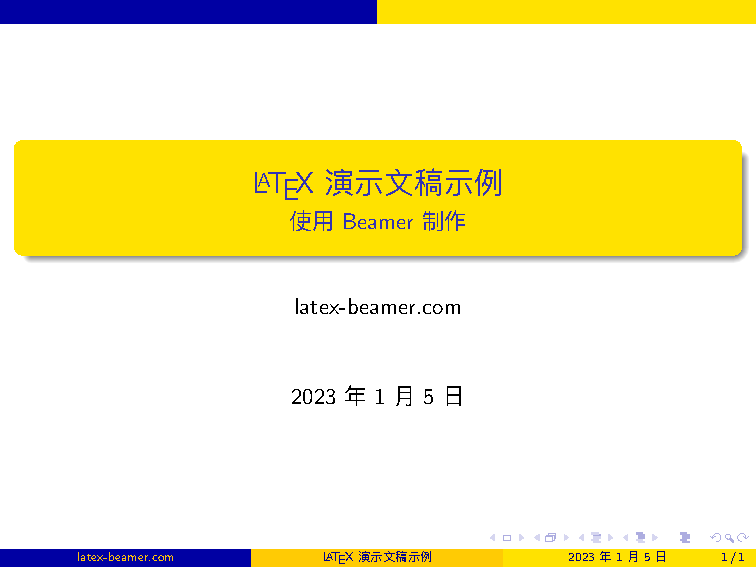
\includegraphics{examples/beamer/beamertitle01.pdf}

\subsection{多个作者}

In the previous example, we used \verb|\author{}| to add the presenter name to the title page. Using the same command, we can add more authors. Check the following code:

\inputminted[linenos=true]{latex}{examples/beamer/beamertitle02.tex}

Using this line code in the above code, we get the following result:

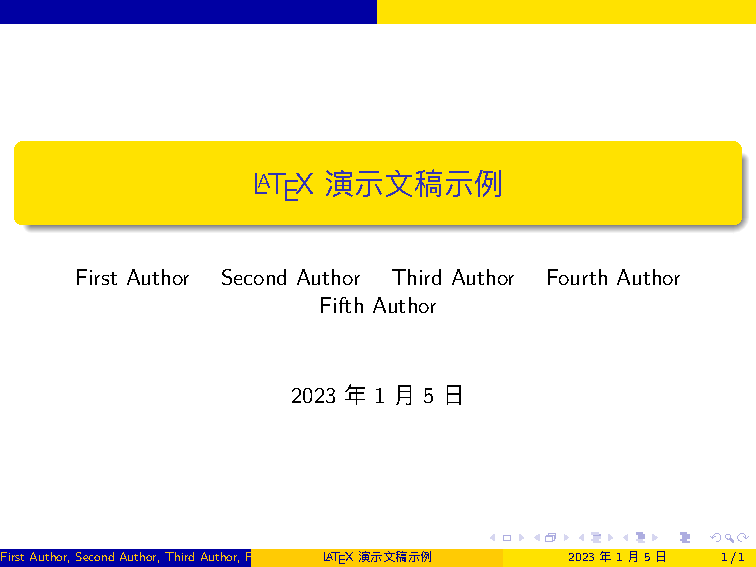
\includegraphics{examples/beamer/beamertitle02.pdf}

对于多个作者的情况,我们使用 \verb|\and| 命令
\footnote{注意:为了保证 first name 和 last name 在换行时不被分开,这里使用 \textasciitilde 来连接。}。

\subsection{作者及单位}

Adding an affiliation can be achieved using the command \verb|\institute{}| to the document preamble.

\inputminted[linenos=true]{latex}{examples/beamer/beamertitle03.tex}

Compiling this code yields the following result:

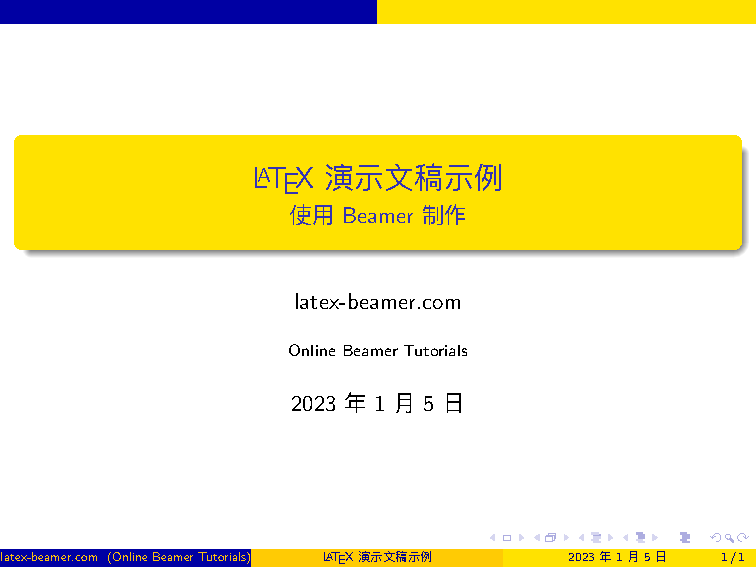
\includegraphics{examples/beamer/beamertitle03.pdf}

If you would like to add multiple lines affiliation, you can simply use \verb|\\| to create a new line.

\subsection{多个作者及单位}

If there are several affiliations or more than one author with different affiliations, we add the command \verb|\inst{}| inside \verb|\author{}| and \verb|\institute{}| commands. Here is an illustrative example of two authors with different affiliations:

\inputminted[linenos=true]{latex}{examples/beamer/beamertitle04.tex}

Here is the obtained result:

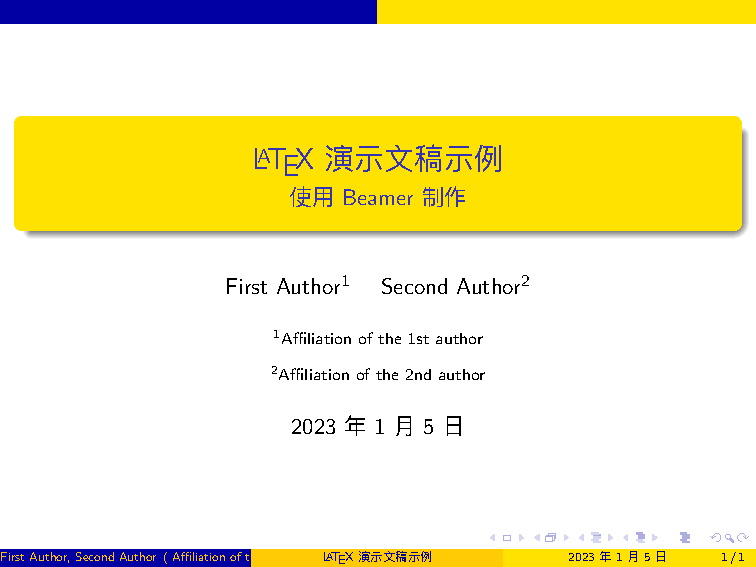
\includegraphics{examples/beamer/beamertitle04.pdf}

\subsection{修改脚注信息}

前面的示例我们看到当标题、作者等信息较长时,无法完整显示。我们可以重新定义脚注显示的信息
\footnote{方括号中可以为空,这样脚注就不显示文本。}:

\inputminted[linenos=true]{latex}{examples/beamer/beamertitle05.tex}

Output:

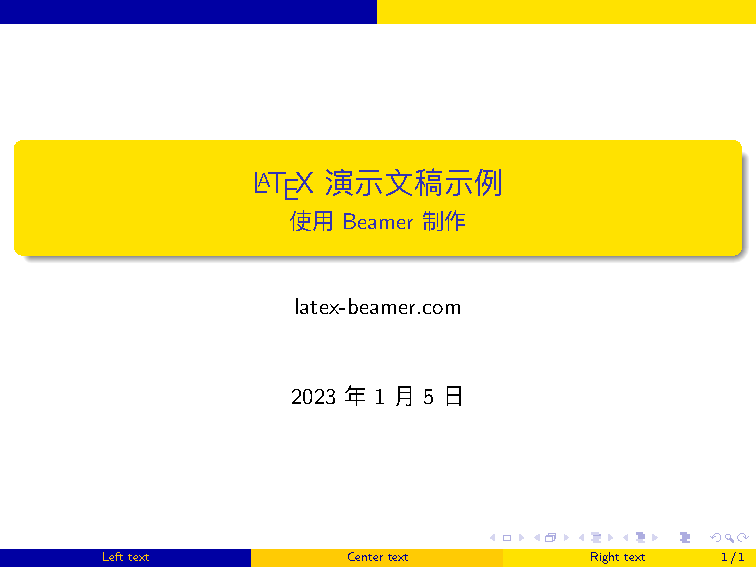
\includegraphics{examples/beamer/beamertitle05.pdf}

% -----------------------------------------------------------------------------
\section{为演示文稿添加 logo}

\subsection{为所以页添加 logo}

Adding a logo in beamer can be achieved using the \verb|\logo{}| command where we include between braces a graphic using \verb|\includegraphics| command, or any text. It should be noted that the logo position is determined by the current theme.

Check the following code:

\inputminted[linenos=true]{latex}{examples/beamer/beamerlogo01.tex}

Compiling this code yields:

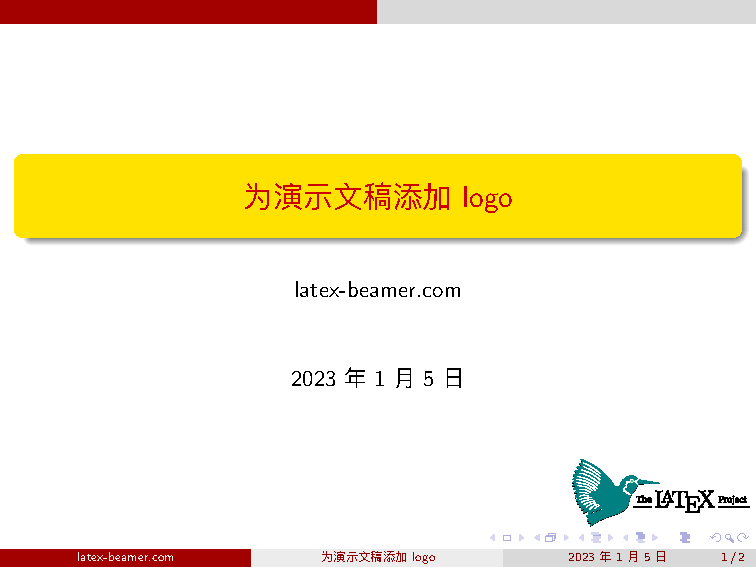
\includegraphics[page=1]{examples/beamer/beamerlogo01.pdf}

\includegraphics[page=2]{examples/beamer/beamerlogo01.pdf}

The logo will appear at the bottom right corner of each slide of this theme.

\subsection{只为封面添加 logo}

In this part, we will learn how to add a logo in the first page only using \verb|\titlegraphic| command. Replacing the above \verb|\logo| line code by the following code:

\inputminted[linenos=true]{latex}{examples/beamer/beamerlogo02.tex}

We get the following output:

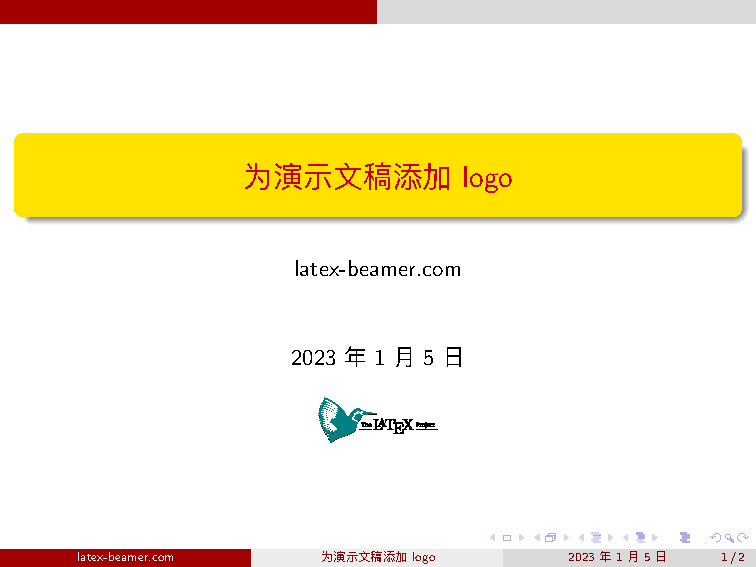
\includegraphics[page=1]{examples/beamer/beamerlogo02.pdf}

\includegraphics[page=2]{examples/beamer/beamerlogo02.pdf}

\subsection{添加多个 logo}

Adding multiple logos can be done by including multiple images using \verb|\includegraphics| command. We can add spacing between logos using \verb|\hspace| command. Here is an illustrative example:

\inputminted[linenos=true]{latex}{examples/beamer/beamerlogo03.tex}

which yields the following title page:

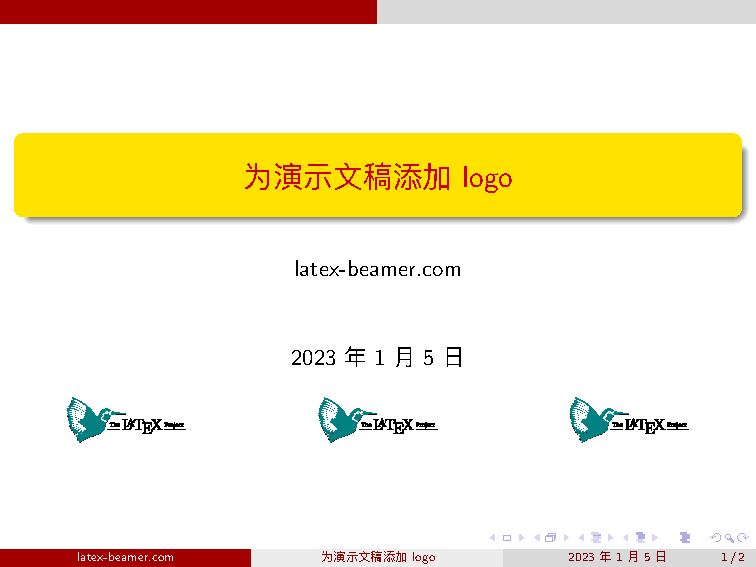
\includegraphics[page=1]{examples/beamer/beamerlogo03.pdf}

\subsection{设置 logo 的位置}

To position our logo at any place of the title page (or slides in general), we will use TikZ package. Here is the steps that we should follow:

\begin{compactitems}
  \item Use \verb|\logo{}| command if we would like to add the logo to all slides or \verb|\titlegraphic{}| command to display it only on the title page.
  \item Create a tikzpicture environment inside one of the above commands (\verb|\logo{}| or \verb|\titlegraphic{}|)
  \item Create a node image and position it with respect to the current slide.
\end{compactitems}
  
Here is an example of top right logo positioning in Beamer:

\inputminted[linenos=true]{latex}{examples/beamer/beamerlogo04.tex}

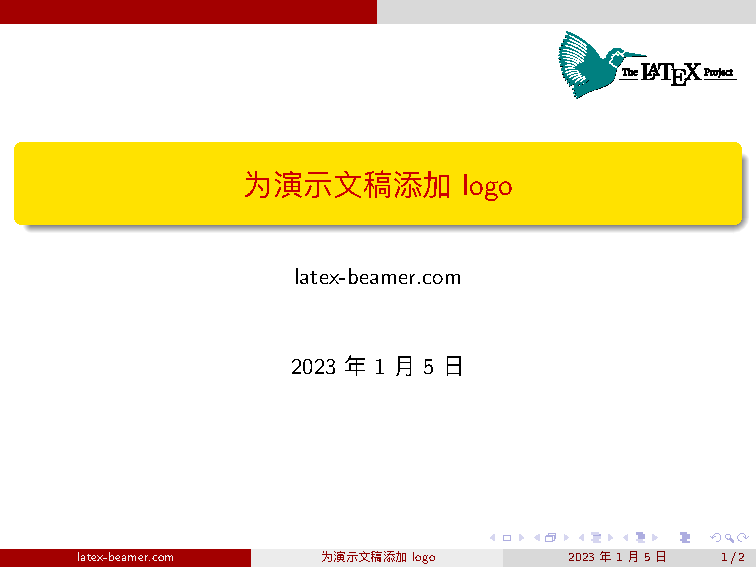
\includegraphics[page=1]{examples/beamer/beamerlogo04.pdf}

Comments:

\begin{compactitems}
  \item \verb|tikzpicture| environment has the following parameters: \verb|overlay| and \verb|remember picture| which are used to create an overlay above the current slide (title page).
  \item a node is created using \verb|\node| command which is positioned at 0.2cm left of the coordinate \verb|(current page.30)|. The latter corresponds to the {\bfseries border point} that makes 30 degrees from the horizontal line passing through the center of the slide.
\end{compactitems}

Here is an example of top left logo positioning in Beamer:

\inputminted[linenos=true]{latex}{examples/beamer/beamerlogo05.tex}

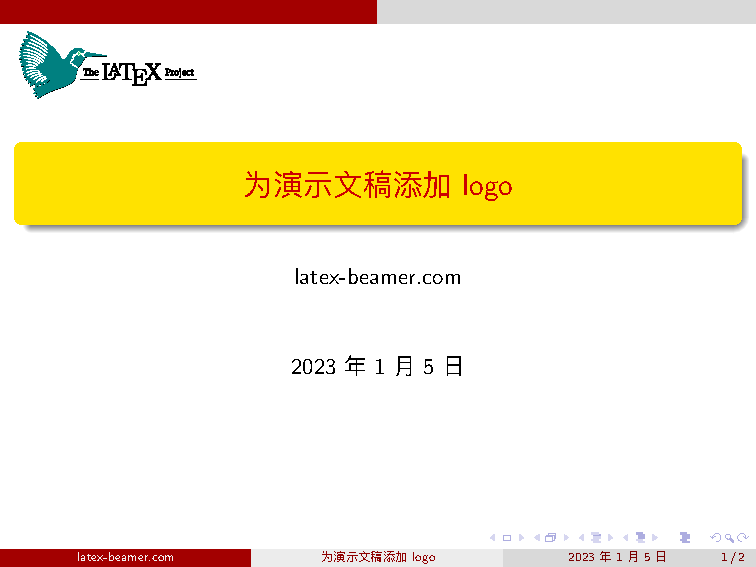
\includegraphics[page=1]{examples/beamer/beamerlogo05.pdf}

where the logo is positioned at 0.2 cm right of the point with coordinates (current page.150)

Here is another example of top left and top right logo positioning in Beamer:

\inputminted[linenos=true]{latex}{examples/beamer/beamerlogo06.tex}

The above code combines the previous line codes and here is the obtained title page:

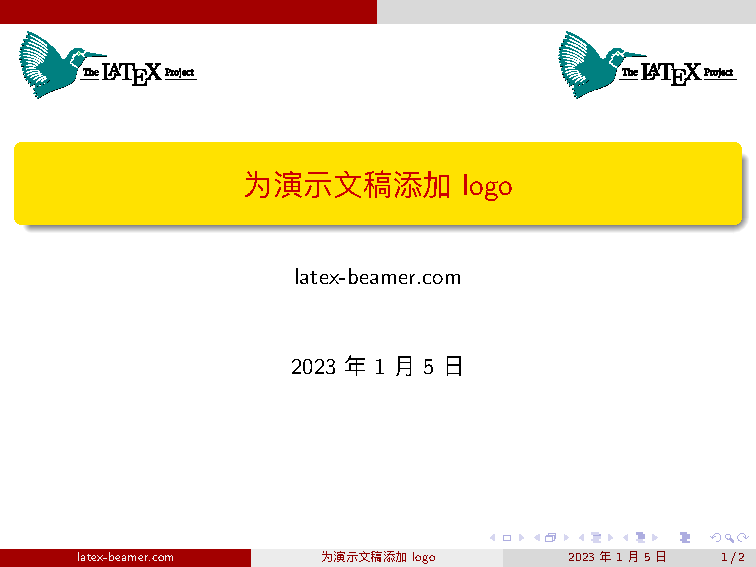
\includegraphics[page=1]{examples/beamer/beamerlogo06.pdf}

We have chosen 30 degrees and 150 degrees, you can choose any value to get the coordinates of the slide border, then use right or left parameters with desired distances to properly position your logo!

% -----------------------------------------------------------------------------
\section{创建目录}

\subsection{创建目录帧}

Creating the table of contents in Beamer can be done with the same manner as in standard {\LaTeX}. The first thing that we should do is to structure our presentation using the commands \verb|\section{}| and \verb|\subsection{}| (\verb|\section*{}| and \verb|\subsection*{}|, to hide it from table of contents). It should be noted that with beamer class these commands will not create a heading at the position where we use them.

\inputminted[linenos=true]{latex}{examples/beamer/beamertoc01.tex}

\begin{remark*}
  这里 \verb|\section|,\verb|\subsection|只是起到锚定作用,并不像 book, article 等文档类一样创建标题,
  真正的标题需要在 \verb|frame| 环境中创建。
\end{remark*}

Compiling this code yields:

\includegraphics[page=2]{examples/beamer/beamertoc01.pdf}

\subsection{在目录中隐藏 {\ttfamily subsection} 标题}

Sometimes, it’s convenient to remove all subsections from the table of contents. This can be done easily using the following line code:

\inputminted[linenos=true]{latex}{examples/beamer/beamertoc02.tex}

we get the following presentation outline:

\includegraphics[page=2]{examples/beamer/beamertoc02.pdf}

\subsection{高亮显示当前标题}

If you wish to show table of contents with highlighted current section before starting every section you can use the following code:

\inputminted[linenos=true]{latex}{examples/beamer/beamertoc03.tex}

\includegraphics[page=3]{examples/beamer/beamertoc03.pdf}

\subsection{逐节显示目录:{\ttfamily pausesections}}

If we would like to show the table of contents in an incremental way, we can add the option {\ttfamily pausesections} to the \verb|\tableofcontents| command. Here is the corresponding {\LaTeX} code:

\inputminted[linenos=true]{latex}{examples/beamer/beamertoc04.tex}

\includegraphics[page=2]{examples/beamer/beamertoc04.pdf}

% -----------------------------------------------------------------------------
\section{Beamer 的环境}

\subsection{{\ttfamily frame} 环境}

Frame environment creates a presentation slide in beamer. A frame can have one slide or multiple slide depending up on the overlay effects. A frame consists of various components such as headline, footline, frame title, navigation bars, navigation symbols, sidebars, etc. 

\begin{minted}{latex}
% Frame environment
\begin{frame}[options]{Frame Title}{Frame subtitle}
  content
\end{frame}
\end{minted}

The options available under this environment are :

\subsubsection{{\ttfamily allowdisplaybreaks=(break desirability)}}
The break desirability value ranges from 0 to 4. Where, 0 means no breaks at all while 4 means can be broken anywhere. This command is typically of use for inserting formulas. The command makes changes only on the current slide and not to the overlay slides.

\subsubsection{{\ttfamily allowframebreaks=(fraction)}}
The content on the frame will automatically shift to other slides if it fails to fit on one slide. The argument (fraction) is used to specify the percentage of content on a slide. This fraction ranges from 0 to 1. Where, 1 means 100% content is displayed on a single slide. This will, however, spoil the visual appearance and hamper the readability. It is recommended to used 0.5 which will display only 50% on one slide. This option needs to be used with the above option, otherwise it shall make no sense. Used for long equations and bibliographies.

\subsubsection{{\ttfamily b, c, t}}
Here, {\ttfamily b} stands for bottom, {\ttfamily c} stands for center, and {\ttfamily t} stands for top. This option is used to specify the vertical alignment of the frame title. By default, it is always aligned to the top of the frame.

\subsubsection{{\ttfamily noframenumbering}}
This option shall suppress the frame number for the current frame.

\subsubsection{{\ttfamily fragile = singleslide}}
Used to contain fragile text such as a code snippet. The argument ’singleslide’ means that the frame has only one slide.

\subsubsection{{\ttfamily label}}
The label option stores the contents of a frame under the given label. This label can be used to call the same frame at some later point of time in the presentation. \verb|\againframe| command is used for that purpose. Label is also an important option to declare hyperjump targets. This option can be used along with the fragile option.

\subsubsection{{\ttfamily plain}}
This option will suppress all the outer-theme elements, such as headline, footline and sidebars. It can be used for displaying pictures or tables that may occupy full-frame space.

\subsubsection{{\ttfamily shrink}}
This option calculates a factor termed as ’shrink factor’ here. This shrink factor is used to scale the text on the frame. If the text is too large or too small then this option can be used to rescale its size. Beamer will first typeset the whole frame and then evaluate the vertical size of the frame text. If this vertical size is larger than the text height minus the frame title height, beamer computes a shrink factor and scales down the frame text by this factor such that the
frame text then fills the frame completely. This option will active the squeeze option by default.

Finding the shrink factor is more or less a trial and error process. Since the shrinking takes place only after everything has been typeset, shrunk frame text will not fill the frame completely horizontally. For this reason, you can specify a <minimum shrink percentage > like 20. If this percentage is specified, the frame will be shrunk at least by this percentage. Since beamer knows this, it can increase the horizontal width proportionally such that the shrunk text once more fills the entire frame. If, however, the percentage is not enough, the text will be shrunk as needed. The best way to use this option is to identify frames that are overly full, but in which all text absolutely has to be fit on a single frame. Then start specifying first shrink=5, then shrink=10, and so on, until no warning is issued any more. However, using the option will change the font size from slide to slide. This shall distort the appearance of the presentation. It is recommended to avoid the used of this command and rather try to restructure the frames.

\subsubsection{{\ttfamily squeeze}}
This option will result in squeezing of all the vertical spaces in the text. This is mostly used in the enumerate and the itemize environment. It make makes the vertical space in these environments to zero.

\subsection{{\ttfamily abstract} 环境}

In beamer class, {\ttfamily abstract} is defined as an environment and not as a macro. Thus, it should start and end with a begin and end tag. If the \verb|\end{abstract}| tag is not used then the slide contents will be continued to the next slide. This environment will create a title ’abstract’ in the information area of the frame. The margins will be wider than other
environments. Here is the corresponding code:

\begin{minted}{latex}
% Abstract environment
\begin{abstract}
  content
\end{abstract}
\end{minted}

\subsection{{\ttfamily slide} 环境}

The following environment:

\begin{minted}{latex}
% Slide environment
\begin{slide}[options]
  content
\end{slide}
\end{minted}

is similar to the \verb|frame| environment with \verb|fragile=singleslide| option active. The slide environment will typeset the frame in that style. The various options available for this environment are :

\subsubsection{{\ttfamily trans=(prosper transition)}}
This uses the prosper transitions as transition effects while showing the slides.

\subsubsection{{\ttfamily toc=(entry)}}
This option will create an entry of the slide in the table of contents as a subsection. Keeping in mind that display of subsections in table of contents is active.


\subsection{{\ttfamily overlayarea} 环境}

The environment

\begin{minted}{latex}
% Overlay area environment
\begin{overlayarea}<overlay spec>{area width}{area height}
  content
\end{overlayarea}
\end{minted}

is overlay-specification-aware. It is used to dynamically change images or text on different slides using overlay specifications. Everything within the environment will be placed in a rectangular area of the specified size. The area will have the same size on all slides of a frame, regardless of its actual contents. It is used to eliminate the wobbling effect of the slide. The use of the environment with example will be explained in the ”Overlay Specifications” lesson.

\subsection{{\ttfamily overlayprint} 环境}

This environment:

\begin{minted}{latex}
% Overlay print environment
\begin{overlayprint}<overlay specification>[{area width}]
  content
\end{overlayprint}
\end{minted}

is similar to overlayarea environment, except that the area height argument is absent. Here, the area height is equal to the frame height. By default, the area width will be equal to text width. Within this environment, \verb|\only| and \verb|\onslide| commands can be used to replace the text content on different slides.

\subsection{{\ttfamily semiverbatim} 环境}

The text inside this environment is typeset like verbatim text. However, the characters \verb|\|, \verb|{| and \verb|}| retain their meaning.

\begin{minted}{latex}
% semiverbatim environment
\begin{semiverbatim}
  content
\end{semiverbatim}
\end{minted}

\subsection{{\ttfamily theorem} 环境}

As the name suggests, it is used to typeset a theorem. This environment corresponds a block environment. But the block body functions as a math environment. All the equations inserted here will be displayed in italics font style by default and block title will be typeset as boldface font. The [additional text] argument shall be shown along with the block title. By default, no theorem numbers are shown in the presentation modes.

\begin{minted}{latex}
% Theorem environment
\begin{theorem}<〈action specification〉 >[additional text]
  content
\end{theorem}
\end{minted}

\subsection{{\ttfamily proof} 环境}

This environment is used to include a proof in the presentation. The proof will be be typeset inside a block-like environment. The argument (proof name) will replace the block title which is typeset to ”Proof” and display the name of the proof.

\begin{minted}{latex}
% Theorem environment
\begin{proof}<〈action specification〉 >[proof name]
  content
\end{proof}
\end{minted}

The end line of a the proof is symbolized by a qed symbol. By default, this symbol is an empty sqaure. To suppress or change the shape of this symbol, the following command has to be declared in the preamble:

\subsubsection{Remove Q.E.D symbol from Proof}
\begin{minted}{latex}
% Suppress the qed symbol
\def\qedsymbol{} 
\end{minted}

\subsubsection{Modify Q.E.D symbol}
\begin{minted}{latex}
% Filled square symbol
\setbeamertemplate{qed symbol}{$\blacksquare$}
\end{minted}

% -----------------------------------------------------------------------------
\section{Beamer 中的列表}

\subsection{有序列表}

Ordered lists have a numbering before every list item. To create an ordered list in beamer, we use enumerate environment. Inside this environment, the list entries can be updated using the \verb|\item| command. A simple ordered list example is presented below.

\inputminted[linenos=true]{latex}{examples/beamer/beamerlist01.tex}

Compiling this code yields the following frame:

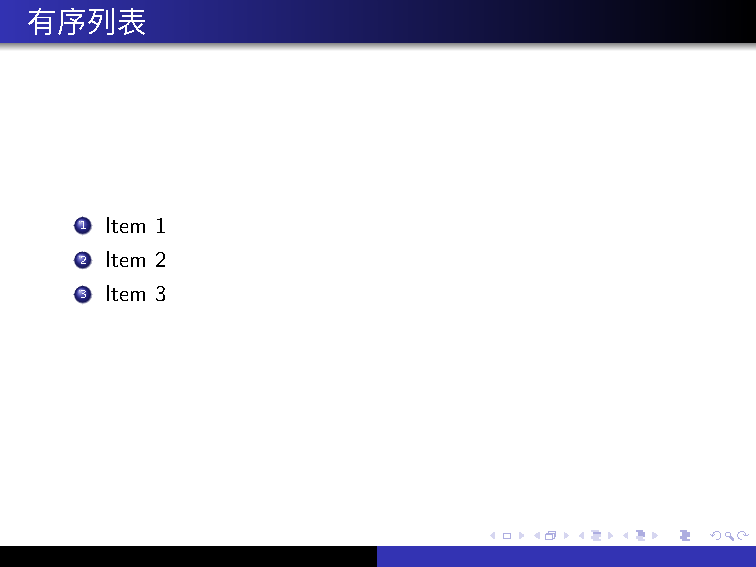
\includegraphics{examples/beamer/beamerlist01.pdf}

\subsection{无序列表}

Unordered lists have a marker, such as a bullet, before every list item. To create an unordered list in beamer, we use the \verb|itemize| environment. Inside this environment, the list entries can be updated using the \verb|\item| command.

A simple unordered list example is presented below.

\inputminted[linenos=true]{latex}{examples/beamer/beamerlist02.tex}

Output:

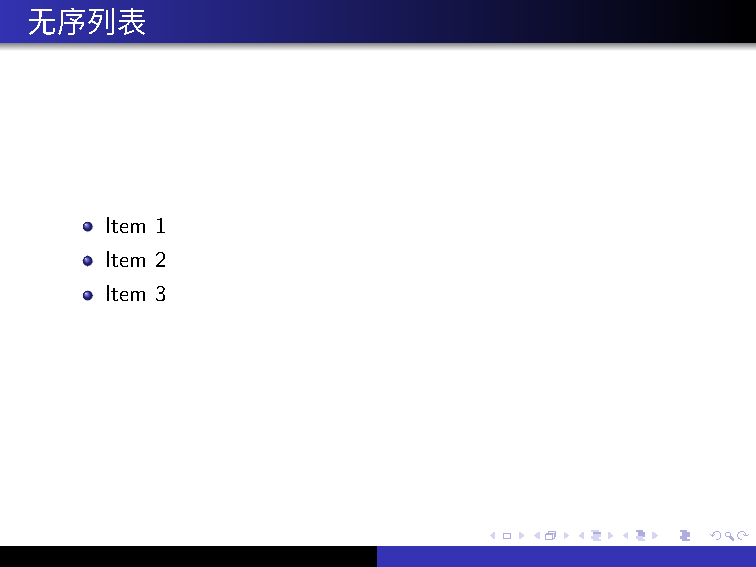
\includegraphics{examples/beamer/beamerlist02.pdf}

\subsection{嵌套列表}

Sometimes you also have to list things, which have some kind of sub-category. For this reason, LaTeX allows you to nest list environments and it will fix the indentation and numbering accordingly.

A simple nested list example is presented below.

\inputminted[linenos=true]{latex}{examples/beamer/beamerlist03.tex}

Compiling this code yields:

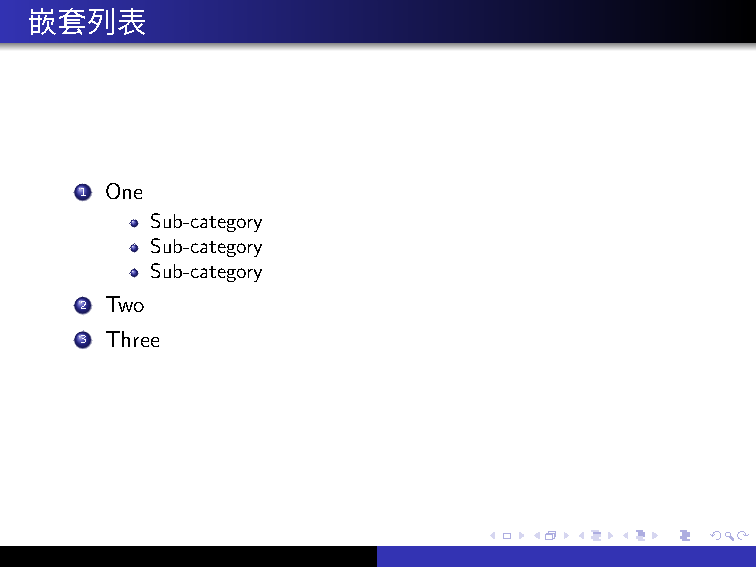
\includegraphics{examples/beamer/beamerlist03.pdf}

\subsection{跨帧列表}

The idea is to define a counter \verb|currentenumi| that stores the value of the last enumerated item in a given frame. Then on the next frame, the \verb|enumi| counter can easily be set to the value of \verb|currentenumi| to continue numbering.

\inputminted[linenos=true]{latex}{examples/beamer/beamerlist04.tex}

which yields the following result:

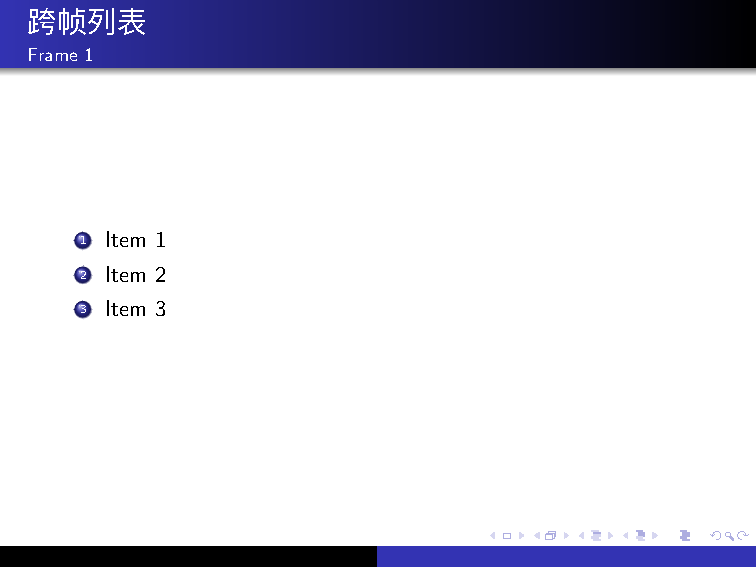
\includegraphics[page=1]{examples/beamer/beamerlist04.pdf}

\includegraphics[page=2]{examples/beamer/beamerlist04.pdf}

\subsection{修改列表项目间距}

The spacing between the list items can be easily altered using the \verb|\vspace| command. The other way to change the spacing globally is to use the following command \verb|\setbeamertemplate|. Here is an illustrative example:

\inputminted[linenos=true]{latex}{examples/beamer/beamerlist05.tex}

Output:

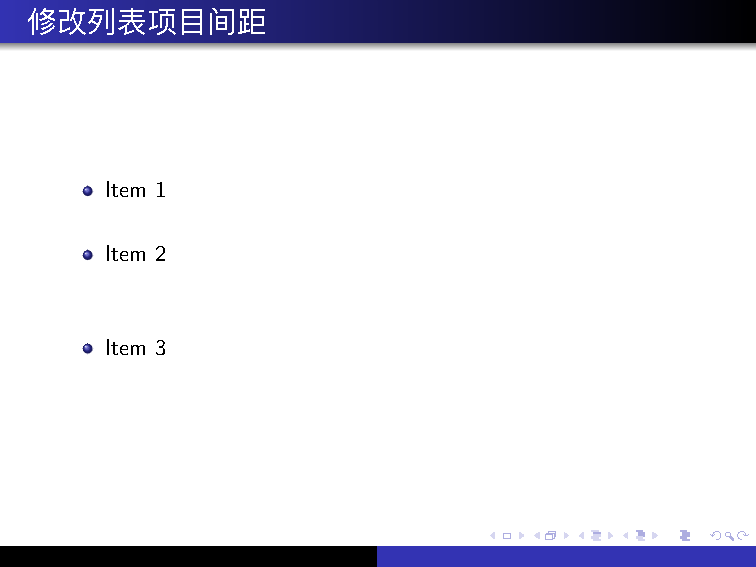
\includegraphics{examples/beamer/beamerlist05.pdf}

Here is another version of spacing between nested lists:

\inputminted[linenos=true]{latex}{examples/beamer/beamerlist06.tex}

Compiling this code yields:

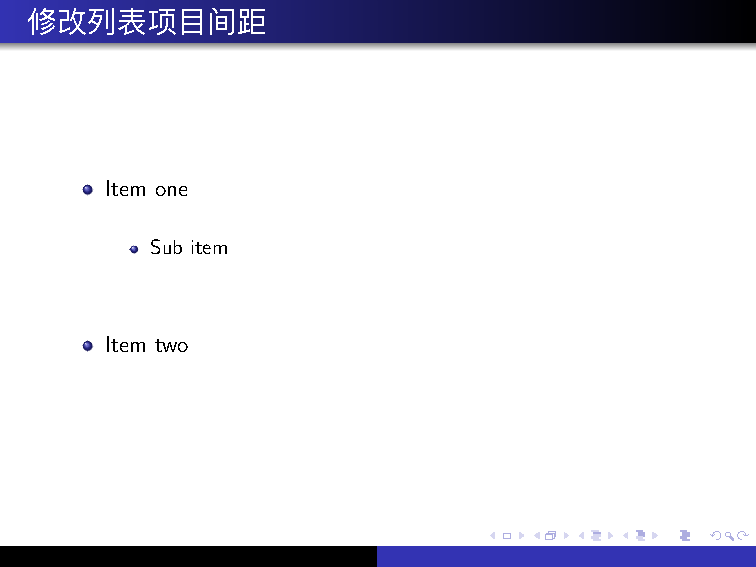
\includegraphics{examples/beamer/beamerlist06.pdf}

\subsection{修改列表项目符号}

There are various templates in beamer to change this itemized list appearance. The command \verb|\setbeamertemplate| is used on itemize items to change the shape of item markers.

\begin{compactitems}
  \item \verb|\setbeamertemplate{itemize items}[default]| : the default item marker is a triangle.
  \item \verb|\setbeamertemplate{itemize items}[circle]| : sets the item marker to a small filled circle.
  \item \verb|\setbeamertemplate{itemize items}[square]| : sets the item marker to a small filled square.
  \item \verb|\setbeamertemplate{itemize items}[circle]| : sets the item marker to a ball shape.
\end{compactitems}

\inputminted[linenos=true]{latex}{examples/beamer/beamerlist07.tex}

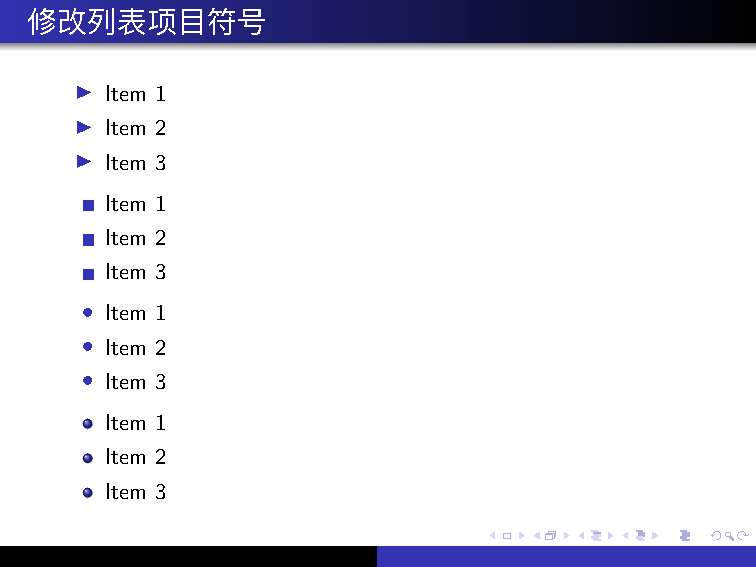
\includegraphics{examples/beamer/beamerlist07.pdf}

使用 pifont 包

\inputminted[linenos=true]{latex}{examples/beamer/beamerlist08.tex}

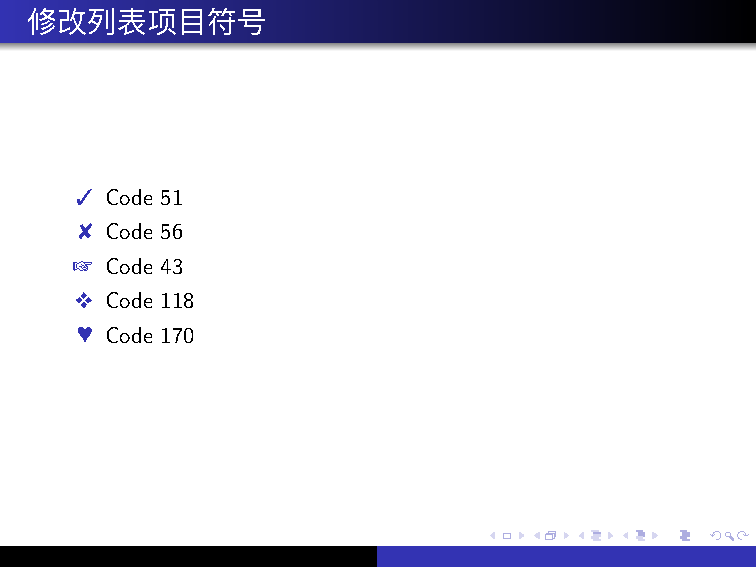
\includegraphics{examples/beamer/beamerlist08.pdf}

\subsection{字母,数字和罗马数字编号}

使用 enumitem 包

Under the enumerate environment, the numbering style can be changed using the enumitem package. From the next example, you can notice that three different styles, alphabet, Roman, and Arabic are used to denote the list item numbers. Meanwhile, you can also separate the enumeration from the item content by enclosing them inside bracket/brackets or a dot.

\inputminted[linenos=true]{latex}{examples/beamer/beamerlist09.tex}

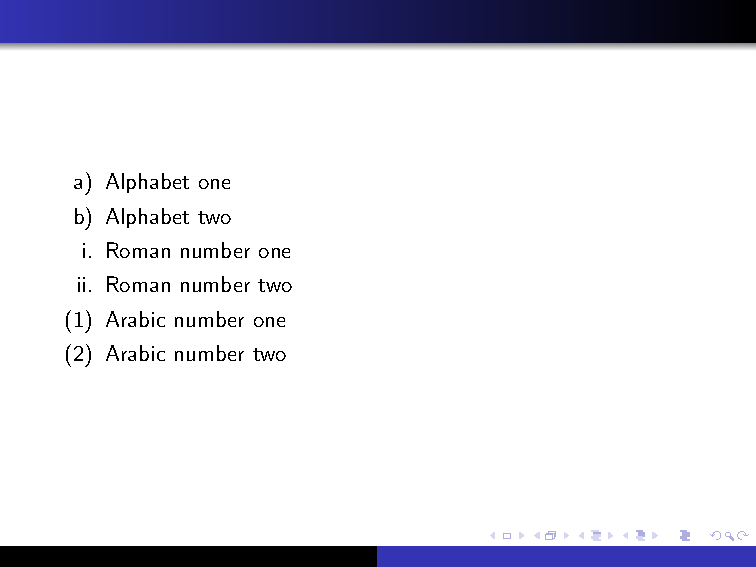
\includegraphics{examples/beamer/beamerlist09.pdf}

% -----------------------------------------------------------------------------
\section{分栏}

\subsection{不同宽度的分栏}

To create columns in beamer, we use the columns environment. Then, at the point to begin a column we use the \verb|\column| command followed by the width of the columns (or {\ttfamily \textbackslash begin\{column\} ...  \textbackslash end\{column\}}).

In the following example, we have created two columns with different widths:

\inputminted[linenos=true]{latex}{examples/beamer/beamercolumn01.tex}

Compiling this code yields:

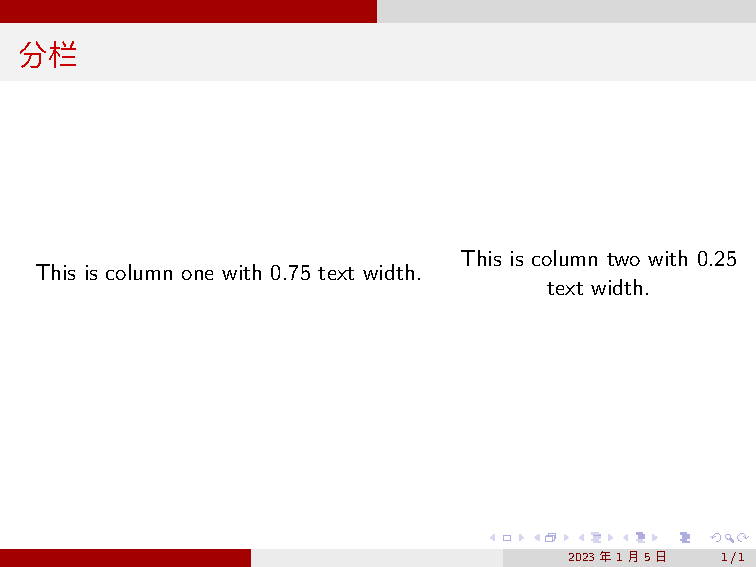
\includegraphics{examples/beamer/beamercolumn01.pdf}

\subsection{文字配图}

With the same manner as above, we can add text and image in the same slide as follows:

\inputminted[linenos=true]{latex}{examples/beamer/beamercolumn02.tex}

Compiling this code yields:

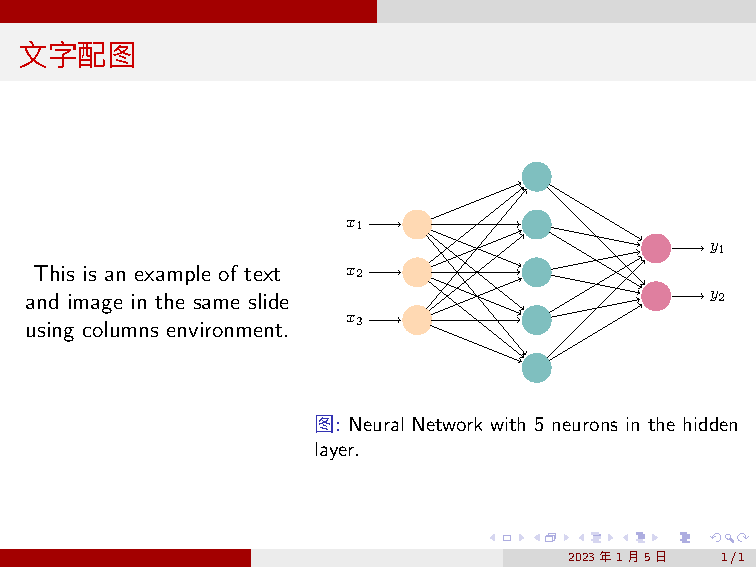
\includegraphics{examples/beamer/beamercolumn02.pdf}

\subsection{垂直分隔线}

To distinctively separate the two (or more) columns from each other we can create a vertical line between them. This can be done simply by adding a \verb|\rule| command in an intermediate column with a small width. In the example below two columns are separated with a vertical line using this method.

\inputminted[linenos=true]{latex}{examples/beamer/beamercolumn03.tex}

Compiling this code yields:

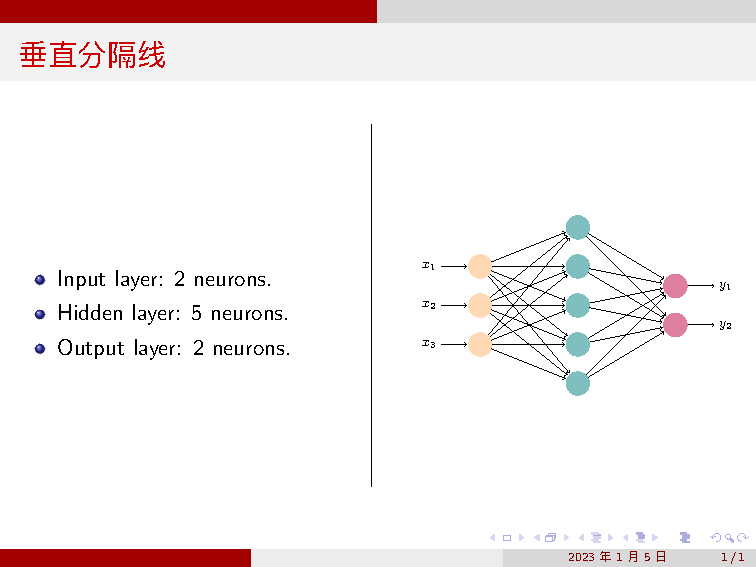
\includegraphics{examples/beamer/beamercolumn03.pdf}

\subsection{垂直方向对齐}

The vertical alignment of column content is very important for the beautification of a presentation. The text and the figures can be placed in three position in a frame, i.e. top, bottom, and center. By specifying [c ], [T], or [b] after beginning the column environment will a automatically position the short content to the center, top, or bottom respectively.

\subsubsection{Top alignment}

\inputminted[linenos=true]{latex}{examples/beamer/beamercolumn04.tex}

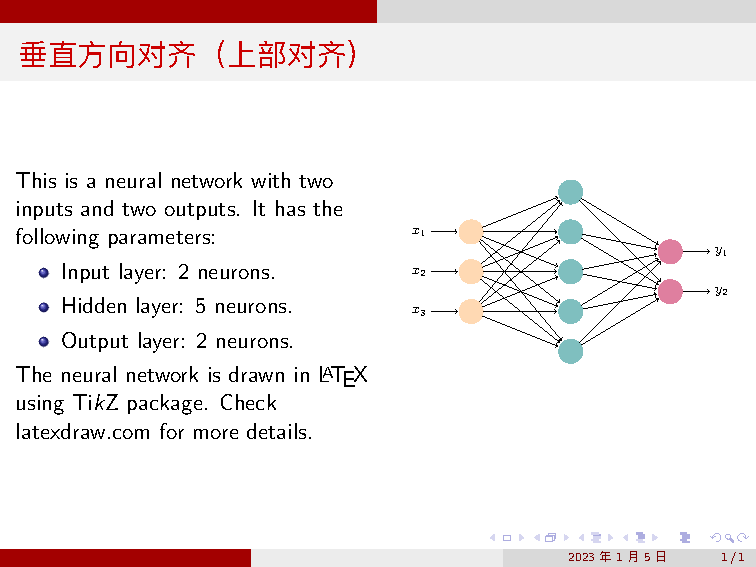
\includegraphics{examples/beamer/beamercolumn04.pdf}

\subsubsection{Center alignment}

\inputminted[linenos=true]{latex}{examples/beamer/beamercolumn05.tex}

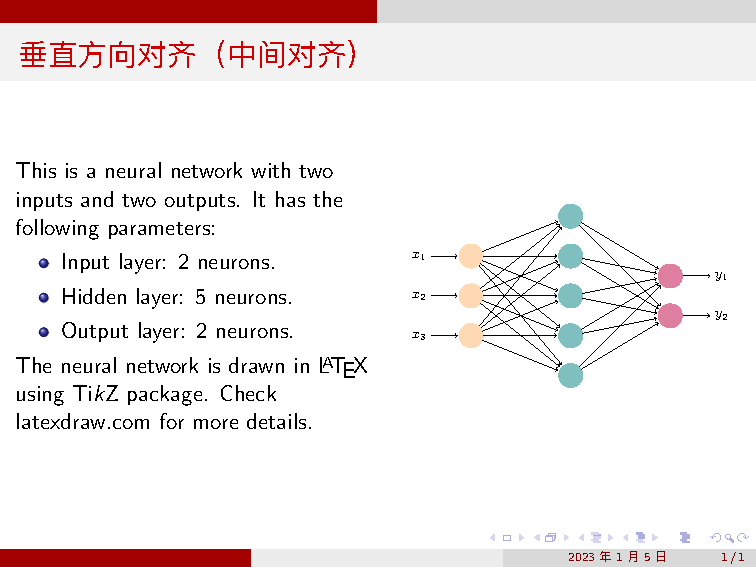
\includegraphics{examples/beamer/beamercolumn05.pdf}

\subsubsection{Bottom alignment}

\inputminted[linenos=true]{latex}{examples/beamer/beamercolumn06.tex}

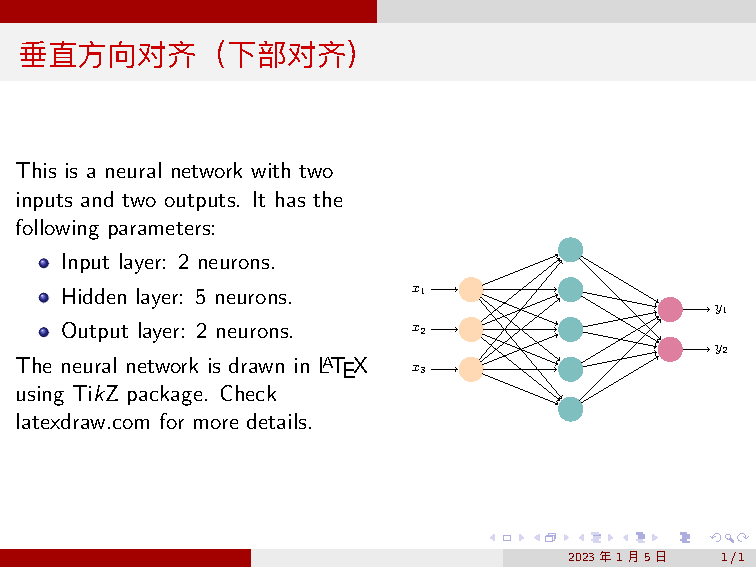
\includegraphics{examples/beamer/beamercolumn06.pdf}

% -----------------------------------------------------------------------------
\section{{\ttfamily block} 环境}

\subsection{创建文字块}

It can be useful to treat some content differently by putting it into a block. In Beamer, we can separate a specific section of text or graphics from the rest of the frame using {\ttfamily block} environment:

\inputminted[linenos=true]{latex}{examples/beamer/beamerblock01.tex}

We used {\ttfamily Madrid} theme for our presentation and inside a frame we added a block environment with title “Block title“. Here is the obtained result:

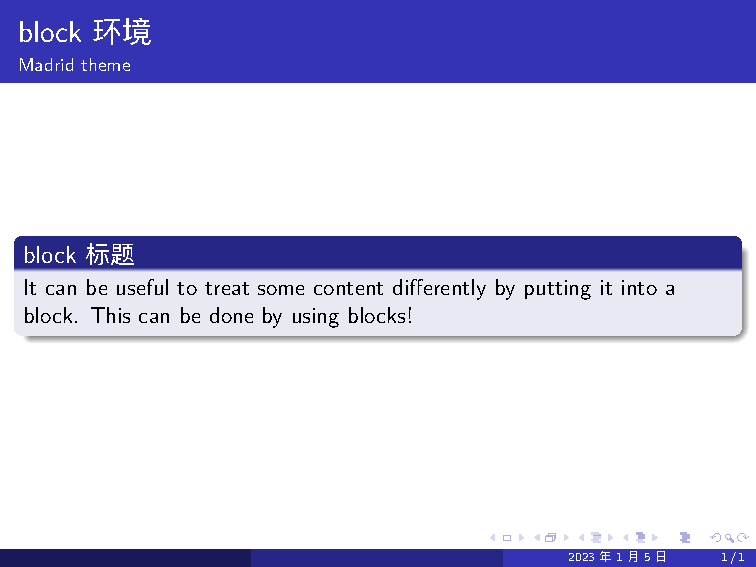
\includegraphics{examples/beamer/beamerblock01.pdf}

It should be noted that the block style depends on the used theme and theme color. Let us consider the same code as above and we change only the them to {\ttfamily Bergen}. The obtained result is shown below:

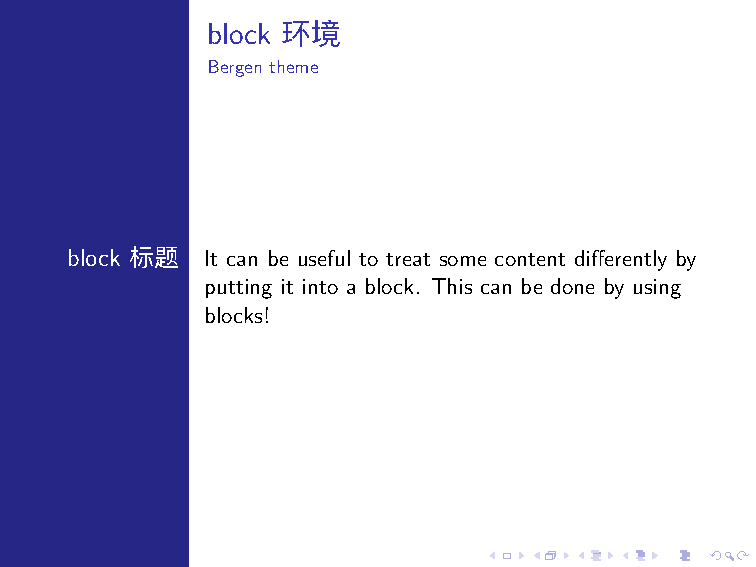
\includegraphics{examples/beamer/beamerblock02.pdf}

\subsection{文字块类型}

There are three basic types of blocks : Standard/Generic block, Alert block, and Example block. There are also special blocks for math environments like Theorem, Definition, Proof, Corollary, Example, etc.

The following table illustrates different blocks with sample code syntax in beamer:

\begin{table}[!h]
\begin{center}
\caption{examples/beamer/Beamer 文字块类型}
\begin{tabular}{cc}
  \toprule
  Content type &  Block\\
  \midrule
  Generic/Standard	& {\ttfamily block}\\
  Highlighted Alert	& {\ttfamily alertblock}\\
  Examples 1	& {\ttfamily exampleblock}\\
  Examples 2	& {\ttfamily example}\\
  Theorems	& {\ttfamily theorem}\\
  Definition	& {\ttfamily definition}\\
  Proofs	& {\ttfamily proof}\\
  Lemmas	& {\ttfamily lemma}\\
  Corollaries	& {\ttfamily corollary}\\
  \bottomrule
\end{tabular}
\end{center}
\end{table}

Here is an example code using different types of blocks in a Beamer presentation:

\inputminted[linenos=true]{latex}{examples/beamer/beamerblock03.tex}

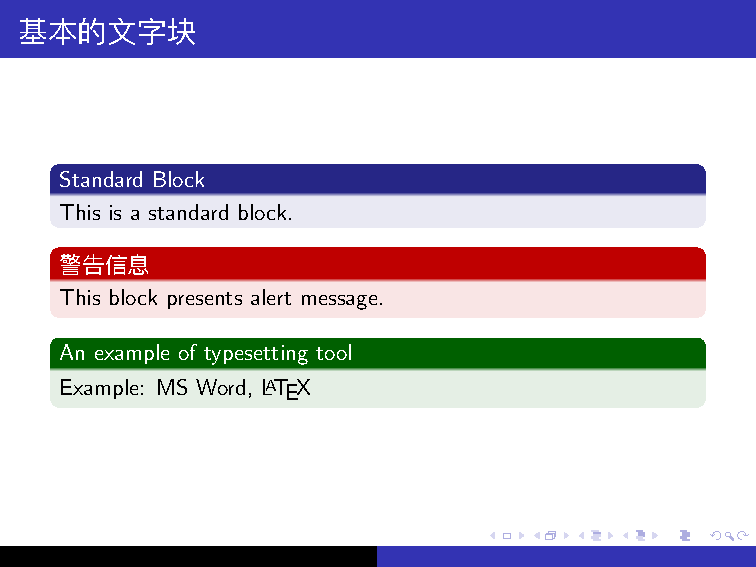
\includegraphics[page=1]{examples/beamer/beamerblock03.pdf}

\includegraphics[page=2]{examples/beamer/beamerblock03.pdf}

\includegraphics[page=3]{examples/beamer/beamerblock03.pdf}

Using {\ttfamily Boadilla} theme instead of {\ttfamily Copenhagen}, we get the following style for different beamer blocks:

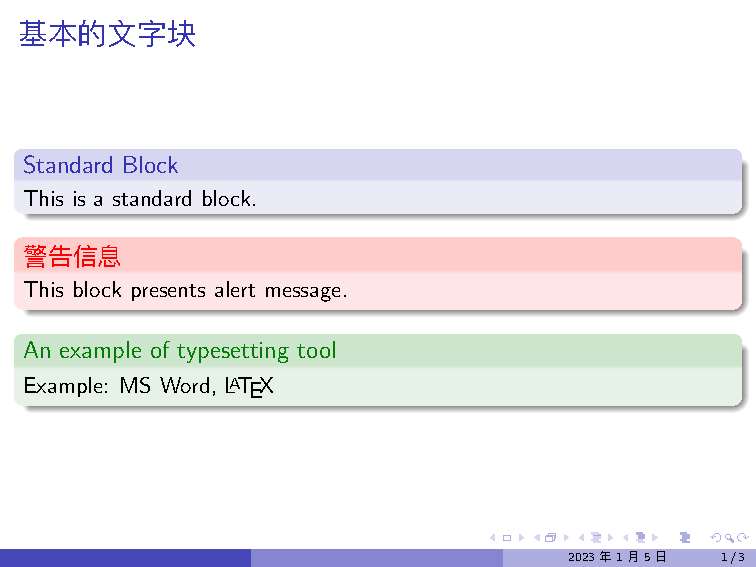
\includegraphics[page=1]{examples/beamer/beamerblock04.pdf}

\includegraphics[page=2]{examples/beamer/beamerblock04.pdf}

\includegraphics[page=3]{examples/beamer/beamerblock04.pdf}

\subsection{自定义文字块}

We can modify blocks’ shapes by playing with the command: \verb|\setbeamertemplate{blocks}[Options]|. Here are available pre-defined options for this command:

\begin{compactitems}
  \item \verb|[default]|: This default value typesets the block title on its line.
  \item \verb|[rounded]|: makes the blocks’ corners rounded.
  \item \verb|[shadow=true]|: If the shadow is set as true, a shadow is portrayed behind the block.
\end{compactitems}

Here is an illustrative example:

\inputminted[linenos=true]{latex}{examples/beamer/beamerblock05.tex}

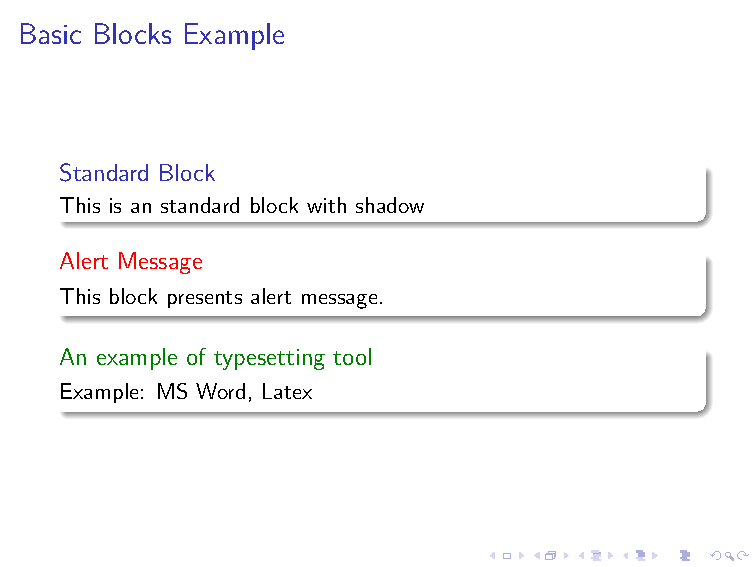
\includegraphics{examples/beamer/beamerblock05.pdf}

\subsection{修改文字块颜色}

From above, we know that blocks’ style depends on the used theme and In this part, we will learn how to change the blocks colors without changing the theme.

For each block (e.g. \verb|alertblock| ), we distinguish two parts: the \verb|title| and the \verb|body| of the block. For each part, we can change the background color and the foreground color. These options can be modified using the command \verb|\{\ttfamily setbeamercolor}|.

In the next example, we changed colors of standard block, alert block and example block. 

\inputminted[linenos=true]{latex}{examples/beamer/beamerblock06.tex}

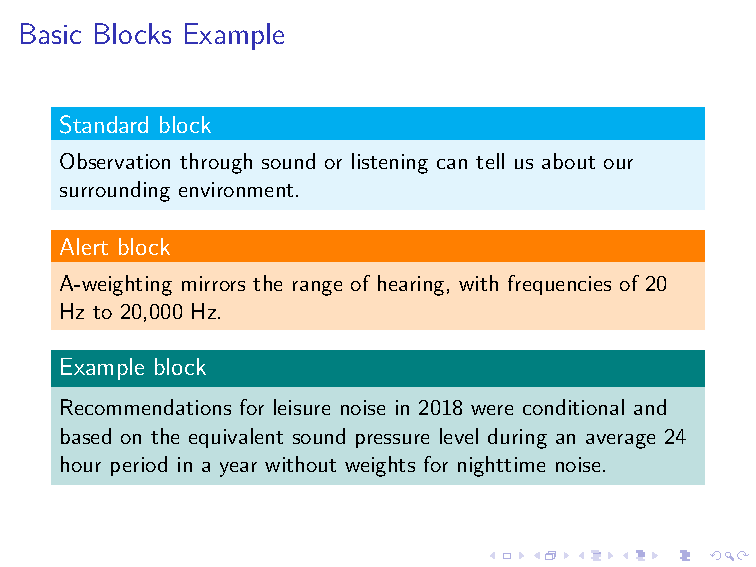
\includegraphics{examples/beamer/beamerblock06.pdf}

% -----------------------------------------------------------------------------
\section{文字格式}

Beamer 中文字格式修饰可以和 {\LaTeX} 其它文档一样,包括粗体、斜体等。
在中文 Beamer 中默认是使用 \verb|\setCJKsansfamily| 定义的字体,
还也可以使用 \verb|\setCJKfamily| 定义中文字体:

\inputminted[linenos=true]{latex}{examples/beamer/beamertextformat01.tex}

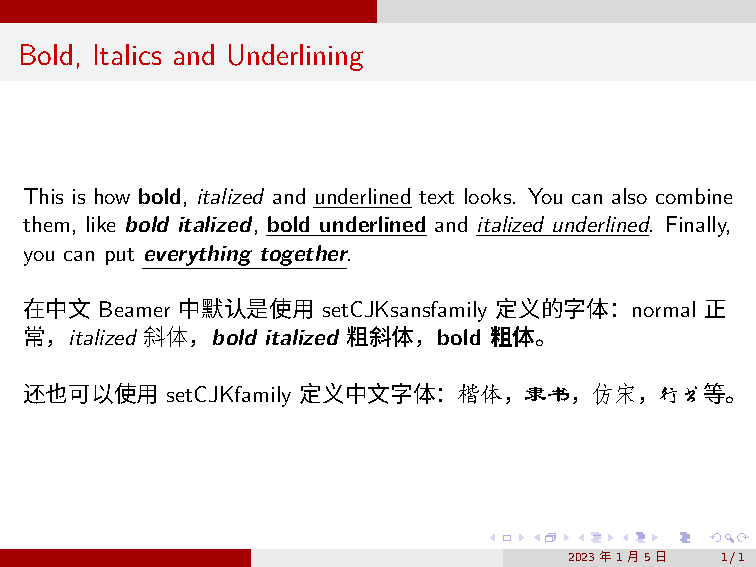
\includegraphics{examples/beamer/beamertextformat01.pdf}

\subsection{Bold Math in Beamer}

As a side note, maybe it is also worth commenting that sometimes we want to use a bold font inside math mode, for instance to denote vectors or matrices. To do so we cannot use the \verb|\textbf| command, but instead we have to load the package bm (which stands for “bold math”) and use the \verb|\bm| command.

\inputminted[linenos=true]{latex}{examples/beamer/beamertextformat02.tex}

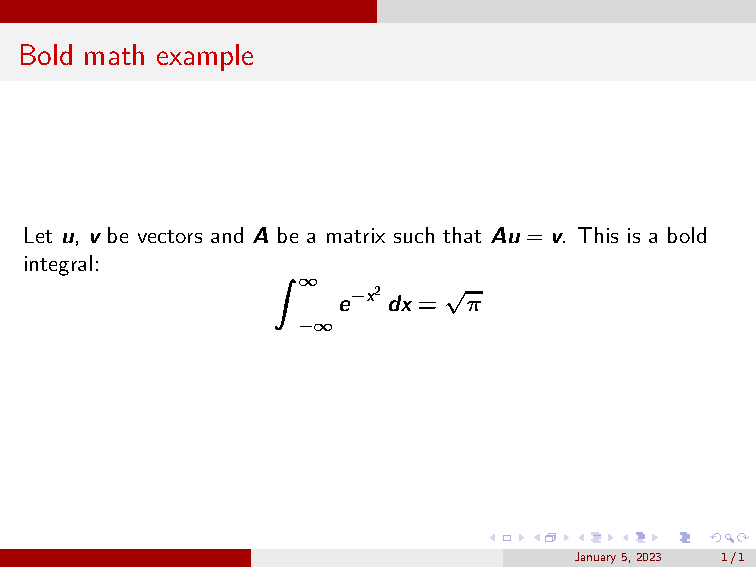
\includegraphics{examples/beamer/beamertextformat02.pdf}

\subsection{Text Decorations in Beamer}

We already saw how to underline text with the \verb|\underline| command that comes with LaTeX. Here we want to go one step further and learn how to do all kinds of “decorations” to our text. To do so, we will be using the ulem package.

This packages mainly changes the way \verb|\emph| works, since instead of emphasizing using the regular italics, it emphasizes the text underlining it. It also introduces the command \verb|\uline| to underline text. By the way, the new underlining is not like the one provided by \verb|\underline|, since the latter will not break at the end of a line, while the former will.

But the ulem package capabilities don’t stop here, since it provides another six more different ways to decorate text.

\begin{table}[!h]
  \begin{center}
  \caption{ulem 宏包命令}
  \begin{tabular}{cc}
    \toprule
    Description	& Command\\
    \midrule
    Underline text solid line	& \verb|\uline|\\
    Double-Underlined text	& \verb|\uuline|\\
    Dashed Underline text	& \verb|\dashuline|\\
    Dotted Underline text	& \verb|\dotuline|\\
    Wavy-Underlined text	& \verb|\uwave|\\
    Strikethrough text	& \verb|\sout|\\
    Struck with Hatching text	& \verb|\xout|\\
    \bottomrule
  \end{tabular}
  \end{center}
\end{table}

对于中文字体修饰可以使用 CJKfntef 宏包,被修饰的文本不要使用 \verb|\CJKfamily| 指定字体,如:\verb|\CJKunderline{{\CJKfamily{楷体}中文}}|。

\inputminted[linenos=true]{latex}{examples/beamer/beamertextformat03.tex}

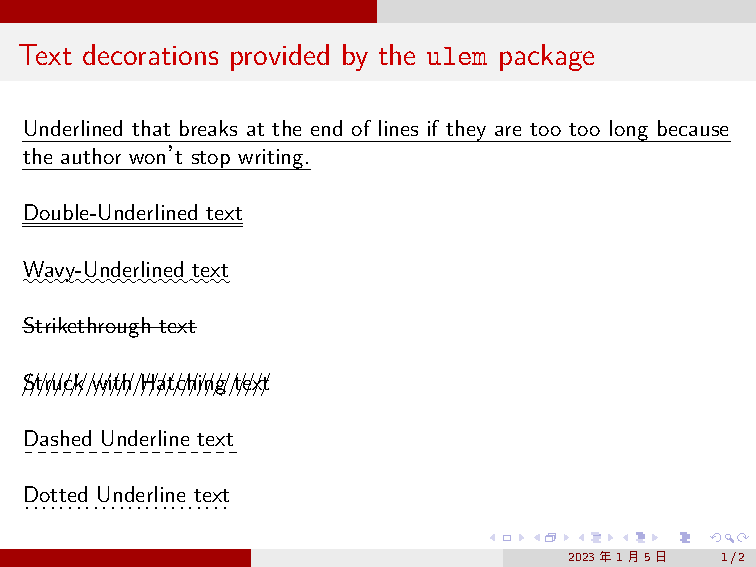
\includegraphics[page=1]{examples/beamer/beamertextformat03.pdf}

\includegraphics[page=2]{examples/beamer/beamertextformat03.pdf}

\subsection{文字对齐}

In general LaTeX documents, paragraphs are usually fully justified, that is, flush both the left and right margins. If you want to change this justification, LaTeX offers the built-in environments flushleft, flushright and center to produce left justified, right justified and centred paragraphs, respectively.

However, there is no built-in environment in LaTeX for fully justified text; and in beamer, by default, the text is left justified. This means that there is no straightforward way of making text fully justified in beamer. This is solved by the ragged2e package, which provides the \verb|\justifying| command. This command, used inside the frame environment, or any other, will produce justified text inside that environment.

The following example shows how to use the different text alignments:

\inputminted[linenos=true]{latex}{examples/beamer/beamertextformat04.tex}

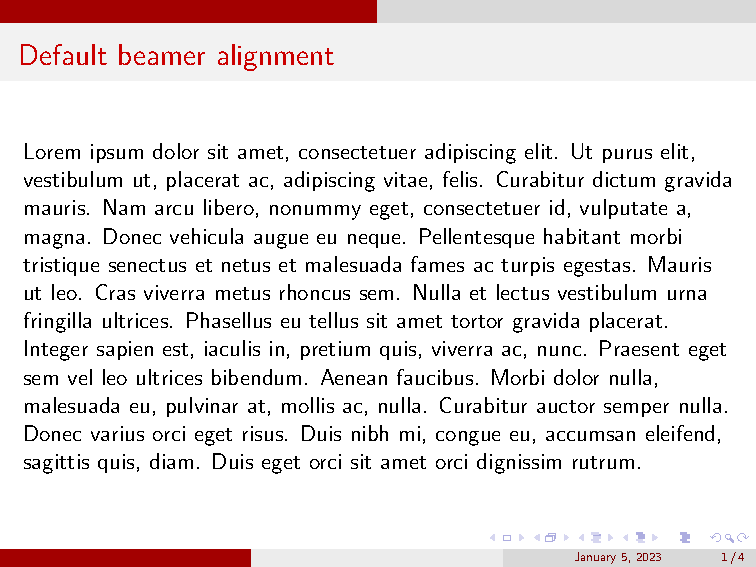
\includegraphics[page=1]{examples/beamer/beamertextformat04.pdf}

\includegraphics[page=2]{examples/beamer/beamertextformat04.pdf}

\includegraphics[page=3]{examples/beamer/beamertextformat04.pdf}

\subsection{调整行距}

If you want to use larger interline spacing in your beamer presentation, you can change its value by using the command:

\verb|\linespread{factor}|

\inputminted[linenos=true]{latex}{examples/beamer/beamertextformat05.tex}

\includegraphics{examples/beamer/beamertextformat05.pdf}

% -----------------------------------------------------------------------------
\section{Beamer 字体}

\subsection{Font Size}

Size is one of the essential properties of a font. The visibility of our content majorly depends on the font size. Predominantly, the Beamer font size was defined in terms of points—for instance, 9 pts, 11 pts, 32 pts, etc .

Beamer has set 11 pts as the normal size of the font. This is the size which is considered as readable from an average distance. Keeping this normal size as datum, other font sizes are defined such as: 
\verb|\tiny|, \verb|\scriptsize|, \verb|\footnotesize|, \verb|\small|, \verb|\normalsize|, \verb|\large|, \verb|\Large|, \verb|\LARGE|, \verb|\huge| and \verb|\Huge|.

The following code highlight different Beamer font size that can be obtained using the above commands:

\inputminted[linenos=true]{latex}{examples/beamer/beamerfont01.tex}

\includegraphics{examples/beamer/beamerfont01.pdf}

Font sizes can also be changed using the beamer class options. We have the sizes: [8pt], [9pt], [10pt], [11pt], [12pt], [14pt], [17pt], [20pt], [bigger], and [small].

Replacing \verb|\documentclass{beamer}| to \verb|\documentclass[14pt]{beamer}|, all font sizes will be shifted where the normal size now is 14pt instead of 11pt. Here is the obtained result:

\includegraphics{examples/beamer/beamerfont02.pdf}

In the process of making our presentation we may face a cramped frame, in which we want to reduce the font size and the line skip, so that all the contents can fit inside. To do so, we can make use of the command

\mint{latex}|\fontsize{<size>}{<vskip>}\selectfont|

Here, and \verb|<vskip>| are TeX dimensions that set the font size and the gap between lines.

This command (as most) will only take effect inside the group or environment in which it is defined; in particular, when put inside a frame environment it will only affect the font sizes of this frame.

Some of the common \verb|<size>| and \verb|<vskip>| units are: point (pt), pica (pc), inch (pt), centimeter (cm) and millimeter (mm).

\begin{minted}{latex}
% Change font size in Beamer
\documentclass{examples/beamer/beamer}

% set a theme
\usetheme{CambridgeUS} 

% Dummy text
\usepackage{lipsum}  

\begin{document}

\begin{frame}{Frame with different font sizes and spacing }{size: 9pt, vskip=10pt}

\fontsize{9pt}{10pt}\selectfont
    
\lipsum[2]
    
\end{frame}
\end{document}
\end{minted}

\subsection{Font Family}

Font family is the second most important property of a Beamer font. Beamer typesets all its text in the \href{https://en.wikipedia.org/wiki/Computer_Modern}{Computer modern} font. There are three types of CM fonts : CM Roman, CM San Serif and CM Typewriter.

Check the following code to get an idea about setting the font family in Beamer:

\inputminted[linenos=true]{latex}{examples/beamer/beamerfont03.tex}

\includegraphics{examples/beamer/beamerfont03.pdf}

We added the option \verb|[fragile]| to be able to use verbatim inside a frame, a more details can be found in \href{https://latex-beamer.com/tutorials/beamer-code/}{“Beamer Code Listing — Syntax highlighter”} lesson.

The other fonts that can be supported by beamer are : Times, Helvetica, Futura.

Besides the font family, beamer has two font series which decide the stroke intensity of the font. The two types of series are : regular and bold. These are obtained using the commands \verb|\mdseries| and \verb|\bfseries|, resepectively.

\subsection{Font Shape and Style}

Beamer supports four types of font shapes: upright, slanted, italics and small caps. Check the example below!

\inputminted[linenos=true]{latex}{examples/beamer/beamerfont04.tex}

\includegraphics{examples/beamer/beamerfont04.pdf}

The upright shape is the default shape for the normal text. The slanted and italics text are seldom used in presentations. The italics font will look same as slant font if the sans-serif font family is used. To have a Times italics effect, the serif font family is mandatory. Italics font shape is used for math. However, the practice of using bold colored text for highlighting is recommended.

The last shape is the small caps. This shape uses smaller versions of the uppercase letters for normal typesetting lowercase letters.

The reading time for the small caps font shape is higher than that for normal text. Thus, making it inadvisable for presentations.

\subsection{Font Weight}

The thickness of the font is referred to as the font weight. The two weights
that are often used are : regular and bold. The bold text is used to create emphasis on a particular topic. The other font weights available in beamer are semibold, ultrabold, thin, and ultrathin.

\subsection{Font Themes}

In this section, we will learn the different pre-defined font themes in beamer. These themes can be used to change the global structure of the presentation.

To change the font family of a theme, we use the command \verb|\usefonttheme| together with one of these font themes:
\begin{compactitems}
  \item \verb|default|,
  \item \verb|dserif|,
  \item \verb|dprofessionalfonts|,
  \item \verb|dstructurebold|,
  \item \verb|dstructureitalicserif|,
  \item \verb|dstructuresmallcapsserif|.
\end{compactitems}

\subsubsection{Theme font: {\ttfamily default}}

The default font theme installs sans serif font for all text of the presentation and installs different font sizes for elements like titles, headlines and footlines, but does not use boldface or italics for “highlighting.”

Consider the following code that loads the default font theme:

\inputminted[linenos=true]{latex}{examples/beamer/beamerfont05.tex}

\includegraphics[page=1]{examples/beamer/beamerfont05.pdf}

\includegraphics[page=2]{examples/beamer/beamerfont05.pdf}

\subsubsection{Theme font: {\ttfamily professionalfonts}}

Using \verb|\usefonttheme{professionalfonts}| instead of \verb|\usefonttheme{default}| in the above code, we get the following result:

\includegraphics[page=1]{examples/beamer/beamerfont06.pdf}

\includegraphics[page=2]{examples/beamer/beamerfont06.pdf}

\subsubsection{Theme font: {\ttfamily serif}}

This theme causes all text to be typeset using the default serif font.

\includegraphics[page=1]{examples/beamer/beamerfont07.pdf}

\includegraphics[page=2]{examples/beamer/beamerfont07.pdf}

\subsubsection{Theme font: {\ttfamily structurebold}}

This font theme will cause titles and text in the headlines, footlines , and sidebars to be typeset in a bold font.

\includegraphics[page=1]{examples/beamer/beamerfont08.pdf}

\includegraphics[page=2]{examples/beamer/beamerfont08.pdf}

\subsubsection{Theme font: {\ttfamily structureitalicserif}}

This theme is similarly as the structurebold font theme, but where structurebold makes text bold, this theme typesets it in italics and in the
standard serif font.

\includegraphics[page=1]{examples/beamer/beamerfont09.pdf}

\includegraphics[page=2]{examples/beamer/beamerfont09.pdf}

\subsubsection{Theme font: {\ttfamily structuresmallcapsserif}}

Again, this theme does exactly the same as the structurebold font theme, only this time text is set using small caps and a serif font.

\includegraphics[page=1]{examples/beamer/beamerfont10.pdf}

\includegraphics[page=2]{examples/beamer/beamerfont10.pdf}

\subsection{Change Math Font style in Beamer}

To make the math in beamer look like the usual {\LaTeX} math, you only have to insert the following declaration in your preamble \verb|\usefonttheme[onlymath]{serif}|.

The following illustration is obtained with the standard Beamer font:

\includegraphics{examples/beamer/beamerfont11.pdf}

\includegraphics{examples/beamer/beamerfont12.pdf}

% -----------------------------------------------------------------------------
\section{Code Listing in Beamer}

\subsection{{\ttfamily fragile} 选项}

If you try to insert code inside a beamer environment like you would do in any LaTeX document, you will get an error. Whether you type the code using the verbatim, minted or listings environment, since they are all different kinds of verbatim text, you will always get the same error!

To make this environments work, you just have to pass the {\ttfamily fragile} option to the frame where the code will go, and everything will work as expected. 

\subsection{使用 minted 宏包显示代码}

To highlight the use of minted package for code syntax highlighting, we consider the following example:

\inputminted[linenos=true]{latex}{examples/beamer/beamercodelisting01.tex}

\includegraphics{examples/beamer/beamercodelisting01.pdf}

你会发现并没有显示行号,原因在于边距的问题,行号在边距之外。见:

\url{https://tex.stackexchange.com/questions/85105/linenumbers-of-minted-are-not-shown-in-beamer-if-i-use-infolines}

This is caused because the numbers are set in the margin, but with the infolines theme, the margin is too small. It does

\mint{latex}|\setbeamersize{text margin left=1em,text margin right=1em}|

modify to 

\mint{latex}|\setbeamersize{text margin left=1cm,text margin right=1cm}|

\inputminted[linenos=true]{latex}{examples/beamer/beamercodelisting02.tex}

\includegraphics{examples/beamer/beamercodelisting02.pdf}

也可以修改 minted 行号的间隔,见:

\url{https://tex.stackexchange.com/questions/525570/minted-line-numbers-outside-frame-and-outside-margin}

\inputminted[linenos=true]{latex}{examples/beamer/beamercodelisting03.tex}

\includegraphics{examples/beamer/beamercodelisting03.pdf}

\subsection{{\ttfamily fragile} 选项详解}

First of all, we have to understand what {\ttfamily fragile} means. This concept has to do with expansion and execution. {\TeX} does these at the same time: first it reads a token, expands it so that only low-level tokens are left and then executes it. But this cycle isn’t always followed: for instance when moving text around this behavior changes.

For instance, when creating a table of contents, since all the chapters, sections and subsections are scattered around your document, but in the end they all end up in the table of contents. To do so, {\TeX}, when reading and executing a \verb|\section| command, will write the current section’s title and number to a .toc file. After all the commands have been parsed, {\TeX} will fill the table of contents based on the data that was collected in the .toc file.

This can represent a problem because the meaning of code changes during {\TeX}'s process, and only when the typesetting is done the actual meaning of some commands can be determined. So when writing data to a file, some expansions must not occur, because they are dependent on the current situation; examples of these are: commands with optional arguments, line breaks, footnotes and inline math.

To deal with this issues, {\TeX} offers the \verb|\protect| command, which can be used to protect fragile commands. In general, the commands that are not fragile (and thus need not protection) are called robust.

But the real question was why did the frame environment need the fragile option? The beamer user manual tells us that using this option the contents of the frame are written to an external file and then read back.

But again one may ask why bother to do so. The truth is that beamer is a very complex package, to the point that it tunes the {\TeX} internal character codes (which are, in turn, one of the most fundamental elements of {\TeX}). When a frame contains fragile text, different internal mechanisms are used to typeset
the frame to ensure that inside the frame the character codes can be reset.

The price of switching to another internal mechanism is that either you cannot use overlays (one of beamer’s main features, and the reason why character codes are changed, since overlays are specified with the symbols < >, which have to change they character codes) or an external file needs to be written and read back (which is not always desirable, because of the extended compilation time, but is the last option available).

It is clear that the character codes are not easily reset when verbatim code appears inside the frame, since the verbatim environments change the character codes, so that you don’t have to use \{\} as delimiters (and thus you can use them inside the command). For instance, I use the delimiters \verb| |(but to write this, I had to use as delimiters + signs).

% -----------------------------------------------------------------------------
\section{图片}

\subsection{{\ttfamily includegraphics} 命令}

\mint{latex}|\includegraphics{file}|

The above command accepts a series of optional arguments, the most important ones being:\verb|height| and \verb|width| to scale the size of the figure.

When only one of these options is set, the other dimension is scaled so that the aspect ratio of the original image is preserved.

Other less common options are also provided:

\begin{compactitems}
  \item \verb|angle| can be passed a rotation angle in degrees, and the image will be rotated this amount counter-clockwise,
  \item \verb|keepaspectratio| is a boolean that forces the image to preserve its aspect ratio.
\end{compactitems}

But if you want to do very fancy things, like both rescaling and rotating an image, be aware that the order in which the options are given matters. The package graphicx interprets the keys from left to right; this means that rotating and then scaling is not the same as scaling and then rotating.

Illustrative example:

In the following example, you can see the difference:

\inputminted[linenos=true]{latex}{examples/beamer/beamerfigure01.tex}

which produces:

\includegraphics{examples/beamer/beamerfigure01.pdf}

Observe how the two images are slightly different.

第 1 个图片是先确定宽度再旋转,第 2 个图片是先旋转再确定宽度。

It should be noted that for the width of images we can use a multiple of the text width via the \verb|\textwidth| command. It is very useful when specifying the dimensions of an image since you can set them to a relative amount of width of the text, without having to worry about low-level \verb|TeX| dimensions.

\subsection{设置图片标题}

Although with this we have a totally functional way of inserting images, in practice we don’t insert them this way, since the image has neither a caption nor a way to reference it. It is more convenient to wrap the \verb|\includegraphics| command inside the figure environment. This is a floating environment that lets us set a caption and a label, and also use position specifiers to control where the image will be placed. However, and this is the main point where beamer differs from other {\LaTeX} documents, \textbf{the position specifiers have no effect in beamer presentations}. They are ignored, and the image is simply placed in the same position as in the source code.

Illustrative example:

In the following example, we show how to use the figure environment to insert images:

\inputminted[linenos=true]{latex}{examples/beamer/beamerfigure02.tex}

Compiling this code yields:

\includegraphics{examples/beamer/beamerfigure02.pdf}

Observe that I have added the declaration:

\mint{latex}|\setbeamertemplate{caption}[numbered]|

in the preamble. The reason for this is that, by default, beamer does not number
the pictures (this is another key difference with the usual {\LaTeX} documents), but since I wanted the figure numbered to reference it, I had to change how the caption looks in the beamer template.

Usually, you will not need the number, since every frame will contain one, at most two, images to be explained, and it is not convenient to use numbers as references throughout a presentation (as it is in a document, where you can easily go back and forth).

\subsection{自定义图片标题}

We have already seen how to slightly change the caption appearance, by adding a number to it or not. But we can further customize it by changing its font size and color. The following example shows the beamer theme options that we have to modify in order to customize our caption:

\inputminted[linenos=true]{latex}{examples/beamer/beamerfigure03.tex}

Compiling this code yields:

\includegraphics{examples/beamer/beamerfigure03.pdf}

\subsection{文字与图片分栏}

It is common to write a frame with a figure next to a certain explanation. For this purpose, we can use beamer’s columns environment, as it is done in the following example:

\inputminted[linenos=true]{latex}{examples/beamer/beamerfigure04.tex}

Compiling this code yields:

\includegraphics{examples/beamer/beamerfigure04.pdf}

Observe that the \verb|\textwidth| command in the line:

\mint{latex}|\begin{column}{0.5\textwidth}|

represents the whole text width of the frame, whereas the \verb|\textwidth| in the \verb|\includegraphics| declaration only represents the text width of the column, which is half of the total text width.

This means that, although we pass to the image the option \verb|width=0.7\textwidth|, it doesn’t take 70\% of the frame, but instead, it takes 70\% of the column.

Although in this case, we accompanied the image with text, any kind of content can be used next to it: text, tables, equations, other images, and so on.

\subsection{图片在帧内的对齐}

Almost all of the time we have been using the figure environment to wrap the \verb|\includegraphics| command so that beamer treats the images as floating objects. However, we can also use the raw \verb|\includegraphics| command, and align it using pure TeX filling commands. The reason behind this is that the \verb|\includegraphics| command just creates a {\TeX}’s box with the image inside it; that is, for the TeX system it is just as any other letter.

To easily centre the image, as we have been doing throughout all the tutorial, we can use the \verb|\centering| command just before \verb|\includegraphics|. However, if we want to left-align the image, we will have to use the command \verb|\hfill| just after including the image, so that all the horizontal space after the image is filled by {\TeX}.

Let me show you a complete minimal example of how this would work:

\inputminted[linenos=true]{latex}{examples/beamer/beamerfigure05.tex}

Compiling this code yields:

\includegraphics[page=1]{examples/beamer/beamerfigure05.pdf}

\includegraphics[page=2]{examples/beamer/beamerfigure05.pdf}

And going further we can apply the same principles for the vertical alignment. By default, the image will be vertically centered. However, we can use the \verb|\vfill| command to fill in vertical space, and thus move the image up and down. If we use it before the image, it will be aligned at the bottom, and if we use it after the image, it will be aligned at the top.

\subsection{图片在帧内任意位置}

The following illustration shows different coordinates of a frame that can be used for absolute positioning of an image using TikZ, check this tutorial for more details!

\href{https://latexdraw.com/how-to-create-a-lined-paper-background-in-latex-using-tikz/}{How to Create a Lined Paper Background in LaTeX using TikZ}

\includegraphics[page=1]{examples/beamer/beamer-frame-position.pdf}

Moreover, we can access the frame border using angles as shown below:

\includegraphics[page=2]{examples/beamer/beamer-frame-position.pdf}

The following code highlights the idea of absolute positioning of an image in Beamer using TikZ package:

\inputminted[linenos=true]{latex}{examples/beamer/beamerfigure06.tex}

Comments:

\begin{compactitems}
  \item We loaded the TikZ package using the command: \verb|\usepackage{tikz}|
  \item We created a TikZ environment inside a frame that we would like to add an image to it. This is achieved by \verb|tikzpicture| environment.
  \item The parameters of the TikZ environment \verb|[remember picture, overlay]| allows us to work on the frame and use absolute positioning.
  \item We created a node at the center of the frame, (current page.center), which has an image a content.
\end{compactitems}

Compiling the above code yields:

\includegraphics[page=1]{examples/beamer/beamerfigure06.pdf}

\includegraphics[page=2]{examples/beamer/beamerfigure06.pdf}

Use left, right, below and above for relative positioning

Now, once you add an image at an absolute position of the frame, you can move it to different directions with respect to the absolute coordinate by adding one of these options: left, right, below or above to the node command!

So to solve the above issue, we can add left option, relative to (current page.east), to the node command.

You can also specify how much left distance by using left=<value> instead of left. 

\inputminted[linenos=true]{latex}{examples/beamer/beamerfigure07.tex}

\includegraphics[page=1]{examples/beamer/beamerfigure07.pdf}

\includegraphics[page=2]{examples/beamer/beamerfigure07.pdf}

You can do the same with right, below and above parameters!

\subsection{修改图片的透明度}

Although we are not going to dive into all of TikZ possibilities, here we are going to explore another functionality that the tikzpicture environment offers: changing the opacity of a figure.

This option is especially interesting when combined with beamer overlay specifications because you can put an image with half its opacity and totally uncover it once you are going to actually talk about it. Even further, you could even decrease the image’s transparency as you get closer to talking about it; this would look very cool.

The following example shows a small implementation of this idea:

\inputminted[linenos=true]{latex}{examples/beamer/beamerfigure08.tex}

\includegraphics[page=1]{examples/beamer/beamerfigure08.pdf}

\includegraphics[page=2]{examples/beamer/beamerfigure08.pdf}

In the above code, we placed the image 1 cm far from the left side of the frame using absolute positioning provided by TikZ. The first version of the image has 30\% opacity and the second one has 100\% opacity.

\subsection{放映设置与图片}

However, if we don’t want such a fancy implementation of opacity, and just want the image to be shown on a given slide, beamer offers us the possibility to pass an overlay specification to the \verb|\includegraphics| command. For example, the declaration:

\mint{latex}|\includegraphics<2-4>[width=\textwidth]{image.png}|

will make the image.png file appear only on slides 2 to 4. 

\subsection{文字环绕图片}

In beamer, we can wrap text around a figure, but not with beamer built-in commands. We have to use the external wrapfig package. In the following example, we use the environment wrapfigure that this package provides to wrap text around a figure:

\inputminted[linenos=true]{latex}{examples/beamer/beamerfigure09.tex}

which produces the following output:

\includegraphics{examples/beamer/beamerfigure09.pdf}

Observe that the {\ttfamily wrapfigure} environment works as the figure environment, in the sense that it makes the image floating, and you can add a \verb|\caption| and a \label to the figure. However, this command accepts two mandatory arguments:

\begin{compactitems}
  \item the first one is to select where we want the image, it can be r or l, that is, right or left;
  \item the second one is the width to be reserved for the image.
\end{compactitems}

\subsection{文字在图片上}

This can also be done inside a beamer frame, but for that purpose, we have to load the versatile TikZ package. In the following example, we illustrate an easy way to do it:

\inputminted[linenos=true]{latex}{examples/beamer/beamerfigure10.tex}

\includegraphics{examples/beamer/beamerfigure10.pdf}

Let’s dissection the commands used in this example:

\begin{compactitems}
  \item First, we insert an image inside the {\ttfamily tikzpicture} environment as a node called ({\ttfamily image}).
  \item Then, we create a second node where its content is aligned at centre, with options to use a white, huge and bold font. Moreover, we added the option {\ttfamily fill=teal} to fill the node with a teal color.
  \item The key is that we position this node at the centre of the previous one; this position is easily identified with {\ttfamily (image.center)}.
  \item Finally, we create the contents of the node itself, which are just the text string {\ttfamily A beautiful photo!}.
\end{compactitems}

\subsection{图片作为帧的背景}

It is easy to use an image as a frame background in beamer, both globally and locally. In the following example, we put both into practice:

\inputminted[linenos=true]{latex}{examples/beamer/beamerfigure11.tex}

\includegraphics[page=1]{examples/beamer/beamerfigure11.pdf}

\includegraphics[page=2]{examples/beamer/beamerfigure11.pdf}

You can see that the procedure is very intuitive: we just change the background canvas option of the beamer theme to the image that we want to use as background. However, when importing it we should make sure that the size is adjusted to the frame size; otherwise, we will get undesired results.

\subsection{在 Beamer 中插入子图}

With the subcaption package, we can build floating figure environments that contain more than one image, each with its corresponding caption and label. The following example shows how to do so:

\inputminted[linenos=true]{latex}{examples/beamer/beamerfigure12.tex}

Here is the obtained result:

\includegraphics{examples/beamer/beamerfigure12.pdf}

\begin{compactitems}
  \item As you can see, first we create a usual figure environment with its corresponding \verb|\caption| and \verb|\label|.
  \item Then, inside of it, for every subfigure we create a \verb|subfigure| environment, which works essentially as a figure environment, with its corresponding \verb|\includegraphics| to insert the image, its \verb|\caption| and its \verb|\label|.
  \item However, this environment takes a mandatory argument, which is the space to be allocated for the corresponding image (in the previous example, \verb|0.4\textwidth|) and also an optional argument, which determines the positioning of the image inside its allocated space. This argument can be either c, t or b, standing for centre, top and bottom.
  \item By default the image is centred, but in the previous example I have used t and b, so that you can see the difference between the two options.
  \item As you can see, different labels enable us to reference either each one of the subfigures or the figure as a whole.
\end{compactitems}

\subsection{图片作为封面}

\subsubsection{Add image to the slide page (bottom)}

The following minimal working example shows how on can include an image in the title page using \verb|\titlegraphics| command:

\inputminted[linenos=true]{latex}{examples/beamer/beamerfigure13.tex}

Compiling this code yields:

\includegraphics{examples/beamer/beamerfigure13.pdf}

It should be noted that titlegraphics content will move the title page details (title, author, institute, etc) to the above. So sometimes we need to fix also the height of the image in the \verb|\includegraphics| command using height=<value> (e.g. \verb|height=0.5\textwidth|).

\subsubsection{Add image to the slide page (top)}

As the title of a presentation is positioned at the top of a title slide, we can include an image just before the title text inside \title{} command:

\inputminted[linenos=true]{latex}{examples/beamer/beamerfigure14.tex}

Compiling this code yields:

\includegraphics{examples/beamer/beamerfigure14.pdf}

% -----------------------------------------------------------------------------
\section{颜色}

There are two ways to change Beamer colors by setting up your own custom color scheme
\footnote{\url{https://ramblingacademic.com/2015/12/08/how-to-quickly-overhaul-beamer-colors/}}. 
The first method is very quick with {\ttfamily usecolortheme}. 
The second method takes a little bit of tinkering with {\ttfamily setbeamercolor}, but ultimately gives you much more control.

\subsection{Picking Beamer Colors}

The first decision is to pick a color(s). I suggest defining two colors for variety, where one is your primary and one is your secondary. However, only one color is needed for the {\ttfamily usecolortheme} method. There are two ways to pick colors:

\begin{compactitems}
  \item Choose from the list of known Beamer colors. By default, Beamer uses the xcolor package, so you can immediately use any of xcolor‘s pre-defined colors. As of this writing, these colors are listed in Section 2.4 of the official xcolor documentation. For example, the list includes blue, red, green, yellow, etc. A list of 68 colors is available if you load xcolor with the {\ttfamily dvipsnames} option when you load Beamer ({\ttfamily documentclass[xcolor=dvipsnames]\{beamer\}}).
  \item Define your own custom colors. Use the {\ttfamily definecolor} command to assign a custom name and then define the parameters for your color (such as RGB values). This is handy if you want to use a very specific color, as I did.
\end{compactitems}

\section{使用 {\ttfamily usecolortheme} 命令修改 Beamer 颜色}

The command {\ttfamily usecolortheme} can be used to load any of the default Beamer color themes (as displayed on \url{https://www.hartwork.org/beamer-theme-matrix/}). 
But this post is about not using the default color themes. You can use {\ttfamily usecolortheme} with any color you want by applying the color to the {\ttfamily structure} of the presentation.

\mint{latex}|{\ttfamily usecolortheme}[named=UBCblue]{structure}|

Here is a minimal example. I’ve chosen to use the Madrid theme with the {\ttfamily miniframes} outer theme (to add a header) and the {\ttfamily circles} inner theme (to replace the shiny default circles).

\inputminted[linenos=true]{latex}{examples/beamer/beamercolor01.tex}

Compiling this code yields:

\includegraphics[page=1]{examples/beamer/beamercolor01.pdf}

\includegraphics[page=2]{examples/beamer/beamercolor01.pdf}

\section{使用 {\ttfamily setbeamercolor} 命令修改 Beamer 颜色}

If you just want a break from the default color themes, then {\ttfamily usecolortheme} is sufficient. If you want to define exactly what colors are used, then a little more work is required (but not much). My goal was to use UBC’s official colors, so a better solution was needed.

A key find was Thierry Masson’s \href{http://www.cpt.univ-mrs.fr/~masson/latex/Beamer-appearance-cheat-sheet.pdf}{Beamer appearance cheat sheet}. This document lists many of the properties that you can manipulate. Page 1 of the sheet lists things that you can color using {\ttfamily setbeamercolor}. You can play around with it, but here is a quick method to color your entire presentation:

\begin{compactitems}
  \item Set the background color of ALL FOUR palettes to your primary color. Set the foreground color of each palette to your desired text color (most likely black or white).
  \item Set the color of elements that are not defined by the palettes. You can use your primary or secondary color. This might be the hardest step and could take some trial and error to catch everything. The most important one is {\ttfamily structure} (for bullets and numbers in lists). If you have a table of contents, then you will also want to set {\ttfamily section} in {\ttfamily toc}. Anything you don’t catch will appear in the default colour theme.
  \item (optional) Select some palette elements where you would like to see the secondary color and set the color for just those elements. For example, setting {\ttfamily subsection} in {\ttfamily head/foot} to the secondary color has a nice clean appearance in themes that use a header or footer. Why not set a whole palette to the secondary color? You can, but I’ve found that you can end up with some undesirable results in headers.
\end{compactitems}

\inputminted[linenos=true]{latex}{examples/beamer/beamercolor02.tex}

Compiling this code yields:

\includegraphics[page=1]{examples/beamer/beamercolor02.pdf}

\includegraphics[page=2]{examples/beamer/beamercolor02.pdf}

% -----------------------------------------------------------------------------
\section{放映 Overlay}

button

% -----------------------------------------------------------------------------
\section{分发 Handout}
% \chapter{{\LaTeX 编程}}

\section{宏、命令与环境}

\subsection{def vs edef}

这是 plain {\TeX} 定义宏的命令。

def和edef都可以定义宏,其区别是:def定义宏时,其宏体不做展开操作;而edef定义宏时,其宏体需要进行展开操作,直到不能再展开为止。def定义的宏,在实际调用时才进行展开,因此宏定义时可以引用还没有定义的其他的宏;edef定义宏时,由于马上就进行展开操作,因此不能引用还没有定义的宏。无论def定义的宏还是edef定义的宏,在实际调用时都会进行“彻底”的展开操作。

\subsection{命令与环境}

本节内容来自:\url{https://latex.org/forum/viewtopic.php?t=26184}。

{\LaTeX} is a macro language, meaning it is based on macros and you can easily define new macros. The word macro is mainly used for new user commands. On the other hand, macros defined by the kernel or packages are called commands. It is just a strange naming convention.
You can also call them control sequences, as well. Internally, a lot of stuff is going on using the internal \verbum{csname}, \verbum{cs} standing for \textit{control sequence}.

What are environments then? The usual command to define an environment is:

\begin{minted}{latex}
\newenvironment{area}{
  <code beginning the environment>
}{
  <code ending the environment>
}
\end{minted}

To put it in a nutshell, this defines a comman/macro/controlsequence 

\mint{latex}|\newcommand{\area}{<code beginning the environment>}|

and a macro 

\mint{latex}|\newcommand{\endmacro}{<code to end the environment>}|

Of course, this is very simplified and not the real internal code. There is also more going on in the background, for example the test if the environment is already defined and a lot more.

{\LaTeXe} provides \verbum*{newcommand} and \verbum*{newenvironment} in different variations, 
{\TeX} uses \verbum*{def} which is low level and shouldn't be used without care and experience.
The {\LaTeX3} kernel, that is in development for the last 20 years, provides package xparse, 
that you can use with the current version of {\LaTeX}. It provides very powerful extensions and tests and is really worth a look.

\subsection{Difference between classes and packages}

本节内容来自:\url{https://www.overleaf.com/learn/latex/Understanding_packages_and_class_files}

其它参考 StackOverflow
\footnote{\url{https://tex.stackexchange.com/questions/1050/whats-the-difference-between-newcommand-and-newcommand}}
\footnote{\url{https://tex.stackexchange.com/questions/86449/what-is-the-difference-between-newenvironment-and-newenvironment}}
。

The default formatting in {\LaTeX} documents is determined by the class used by that document. 
This default look can be changed and more functionalities can be added by means of a package. 
The class file names have the \textit{.cls} extension, the package file names have the \textit{.sty} extension.

Sometimes it's hard to make a decision when it comes to choose whether to write a package or a class. 
The basic rule is that if your file contains commands that control the look of the logical structure of a special type of document, then it's a class. 
Otherwise, if your file adds features that are independent of the document type, i.e. can be used in books, reports, articles and so on; then it's a package.

For instance, if a company needs branded reports that use a special font and have the logo of the company in the footer; you need a new class.

If the company needs a new command that makes easier to highlight important sentences within a document, a new package will work in this scenario.

\section{创建命令 \protect\verbum*{newcommand}}

基本形式:

\mint{latex}|\newcommand{<命令名>}[<参数个数>][<第一个参数的默认值>]{<定义>}|

\verbum*{newcommand} 有如下的三种使用方式:

\subsection{定义无参数的命令}

这是 \verbum*{newcommand} 最简单的使用方式,比如:

\begin{texcode}
\newcommand\lipsum{Lorem ipsum dolor sit amet}
A common form of Lorem ipsum reads: \lipsum ...
\end{texcode}

当然,\verbum{<定义>}部分可以是一段代码,需要使用 \mintinline{latex}{\begin{group} ... \end{group}} 
或 \verbum{\{\}}来包含这段代码。

\subsection{定义有参数的命令}

定义有参数命令的通用形式为:

\mint{latex}|\newcommand{<命令名>}[<参数个数>]{<定义>}|

方括号中定义了命令的参数个数(最多9个),在命令的定义中,可以使用 \#1 引用第一个参数,\#2 引用第二个参数,以此类推,比如:

\begin{texcode}
\newcommand\pyth[3]{\ensuremath{#1^2 + #2^2 = #3^2}}
在平面几何中, 勾股定理是指一个直角三角形的三边满足公式: \pyth{a}{b}{c}.
\end{texcode}

\subsection{定义带默认值参数的命令}

在定义带参数的命令时,{\LaTeX} 也允许其中的一个参数有默认值,即在调用命令时可以不给出这个参数,直接取用该参数的默认值。这个带默认值的参数,在LaTeX中永远使用 \#1 来引用。
定义带默认值参数的命令的通用形式为: 

\mint{latex}|\newcommand{<命令名>}[<参数个数>][<第一个参数的默认值>]{<定义>}|

需要特别注意的是,当调用这个命令时,使用 \verbum{\{\}} 形式给出的参数列表要比定义命令时少一个,
即带默认值的参数不能以 \verbum{\{\}} 的形式给出。
要么使用参数的默认值,这样就不需要给出 \#1 这个参数;
要么使用 \verbum{[]} 在其他参数前面重新定义默认值。 
显然,带默认值参数的命令,至少有一个参数。 
下面是一个具有一个参数且有默认值的命令:

\inputlatexcode{snippets/programming/command-with-optional-parameters.tex}

\subsection{\protect\verbum*{makeatletter} 和 \protect\verbum*{makeatother}}

有编程经验的人很容易写出下面的代码:

\begin{minted}{latex}
\newcommand\str1{Lorem ipsum dolor sit amet}
\newcommand\str2{consectetur adipiscing elit}
\end{minted}

当这段代码出现在导言区时,会出现错误:\mintinline{latex}{LaTeX Error: Missing \begin{document}};
当出现在 \verbum{document} 环境内部时,定义无效但不会报错。

{\LaTeX} 的命令和 {\TeX} 的命令一样,
只允许普通字符(26个字母的大小写形式)作为命令的名称,
不允许出现数字、特殊字符等。当然,这不是一个不可逾越的鸿沟。
本质上来说,只要 catcode=11 的字符都可以作为命令的名称,
因此只要修改字符的 catcode 为11,这个字符就可以出现在命令的名称中。
LaTeX的内部命令中,\verbum*{makeatletter} 命令的实质就是修改字符@的catcode为11,
这样@就可以出现在命令名称中了。\verbum*{makeatother} 重新修改@的catcode为12,
不允许@出现在命令的名字中。

\section{创建环境 \protect\verbum*{newenvironment}}

\subsection{基本用法}

定义环境的一般形式:

\mint{latex}|\newenvironment{<环境名>}[<参数个数>][<第一个参数的默认值>]{<环境前定义>}{<环境后定义>}|

其中:
\begin{itemize}
  \item \verbum{<环境前定义>}中的代码在环境开始时执行,也即 \mintinline{latex}{\begin{<环境名>}} 时执行。在这段代码中,你能够使用参数,与命令定义类似。
  \item \verbum{<环境后定义>}中的代码在环境结束时执行,也即 \mintinline{latex}{\end{<环境名>}} 时执行。在这段代码中,你不能使用参数,解决方法见下文。
\end{itemize}

下面的代码将产生错误: \mintinline{latex}{Illegal parameter number in definition of \endnormaltext}。

\begin{minted}{latex}
\newenvironment{normaltext}[1][\itshape]%
  {#1}%
  {\typeout{what was #1, again?}}
\end{minted}

解法方法是将参数暂时保存:

\begin{texcode}
\newenvironment{normaltext}[1][Intro]%
  {#1\par%
   \newcommand{\foo}{#1}}%
  {\par what was \foo, again?}

\begin{normaltext}
Lorem ipsum dolor sit amet
\end{normaltext}
\end{texcode}

如何获取环境内容?解决方法:使用 envrion 包或者如 compositor 包中的 \verbum{texcode} 环境实现,先输出到文件,再读入该文件。

\subsection{环境的编号}

下面自定义一个定理环境
\footnote{\url{https://www.overleaf.com/learn/latex/Environments}}
\footnote{\url{https://www.overleaf.com/learn/latex/Counters}}:

\begin{texcode}
\newcounter{theorema}[section]
\counterwithin*{theorema}{section}
\newenvironment{theorema}[1][]{\refstepcounter{theorema}\par\medskip
    \noindent \textbf{定理~\thesection.\thetheorema. #1} \rmfamily}{\medskip}

\begin{theorema}[勾股定理]
直角三角形的两条直角边的平方和等于斜边的平方
\end{theorema}

\begin{theorema}
两条直线被第三条直线所截,如果内错角相等,那么这两条直线平行。
\end{theorema}
\end{texcode}

\section{创建宏包}

参考 \cite{CLSGUIDE}、\cite{WIKIBOOKS} 、\cite{COMPANION} 和 Overleaf 教程\footnote{\url{https://www.overleaf.com/learn/latex/Writing_your_own_package}}
{\LaTeXe} 对选项 Options 的支持只是选择性, 如果需要键值对选项需要使用 kvoptions,或 xkeyval,或pgfkeys 包。

\subsection{宏包的结构}

The structure of all package files can be roughly described in the next four parts:

\begin{description}
  \item[Identification] The file declares itself as a package written with the {\LaTeXe} syntax.
  \item[Preliminary declarations] Here the external packages needed are imported. Also, in this part of the file the commands and definitions needed by the declared options are coded.
  \item[Options] The package declares and processes the options.
  \item[More declarations] The main body of the package. Almost everything a package does is defined here.
\end{description}

In the next subsections a more detailed description of the structure and a working example will be presented.

我们先看一个实例,在该实例中我们创建了一个名为 colorbox 的宏包,并且使用了 xkeyval 包来解析键值对参数:

\inputminted{latex}{examples/programming/create-packages.tex}

\subsubsection{Identification}

There are two simple commands that all packages must have:

The command \mintinline{latex}|\NeedsTeXFormat{LaTeX2e}| sets the {\LaTeX} version for the package to work. 
Additionally, a date can be added within brackets to specify the minimal release date required.

The command \mintinline{latex}|\ProvidesPackage{<package name>}[...]| identifies this package as 
\verbum{<package name>} and, inside the brackets, the release date and some additional information 
is included. The date should be in the form YYYY/MM/DD.

\subsubsection{Preliminary declarations}

Most of the packages extend and customize existing ones, 
and also need some external packages to work. Below, 
some more code is added to the sample package.

The commands in this part either initialize some parameters 
that latter will be used to manage the options, 
or import external files.

The command \verbum*{RequirePackage} is very similar to the 
well-known \verbum*{usepackage}, adding optional parameters 
within brackets will also work. The only difference is that 
the \verbum*{usepackage} can not be used before 
\verbum*{documentclass} command. It's strongly recommended 
to use \verbum*{RequirePackage} when writing new packages or 
classes.

\subsubsection{Options}

To allow some flexibility in the packages a few additional 
options are very useful. The next part in the file handles 
the parameters passed to the package-importing statement.

Below a description of the main commands that can handle the options passed to the package.

The command \verbum*{DeclareOptionX} handles a given option. It takes two parameters, 
the first one is the name of the option and the second one is the code to execute if the 
option is passed.

The command \verbum*{OptionNotUsed} will print a message in the compiler and the logs, t
he option won't be used.

The command \verbum*{Declareoption*} handles every option not explicitly defined. 
It takes only one parameter, the code to execute when an unknown option is passed. 
In this case it will print a warning by means of the next command:
\verbum*{PackageWarning}. See handling errors for a description about what this command does.

\verbum*{CurrentOption} stores the name of the package option being handled at a determined moment.

The command \verbum*{ProcessOptionsX\relax} executes the code fore each option and must be 
inserted after all the option-handling commands were typed. 
There's a starred version of this command that will execute 
the options in the exact order specified by the calling commands.

In the example, if the options \verbum{fcolor} or \verbum{bgcolor} are passed to the \verbum*{usepackage}
 command within the document, the command \verbum*{FrameColor} and \verbum*{BGColor} are redefined. 
 Both colours and the default grey colour were defined in the preliminary declarations after importing the xcolor package.

\subsubsection{More declarations}

In this part most of the commands will appear. Below you can see the full package file.

This package defines a new command \verbum*{textbox}, that prints the words in a special colour.

To fully understand each command see the reference guide and the links in the further reading section.

Below, a document that uses the package.

\subsection{Handling errors}

When it comes to develop new packages it's important to handle possible errors to let know the user that something went wrong. There are four main commands to report errors in the compiler.

\mintinline{latex}|\PackageError{package-name}{error-text}{help-text}|. Takes three parameters, each one inside braces: the package name, the error text which is going to be displayed (the compilation process will be paused), and the help text that will be printed if the user press "h" when the compilation pauses because of the error.

\mintinline{latex}|\PackageWarning{package-name}{warning-text}|. In this case the text is displayed but the compilation process won't stop. It will show the line number where the warning occurred.

\mintinline{latex}|\PackageWarningNoLine{package-name}{warning-text}|. Works just like the previous command, but it won't show the line where the warning occurred.

\mintinline{latex}|\PackageInfo{package-name}{info-text}|. In this case the information in the second parameter will only be printed in the transcript file, including the line number.

\subsection{Reference guide}

List of commands commonly used in packages and classes

\mintinline{latex}|\newcommand{name}{definition}|. Defines a new command, the first parameter is the name of the new command, the second parameter is what the command will do.

\mintinline{latex}|\renewcommand|. The same as \verbum*{newcommand} but will overite an existing command.

\mintinline{latex}|\providecommand|. Works just as \verbum*{newcommand} but if the command is already defined this one will be silently ignored.

\mintinline{latex}|\CheckCommand|. The syntax is the same as \verbum*{newcommand}, but instead it will check whether the command exists and has the expected definition, {\LaTeX} will show a warning if the command is now what \verbum*{CheckCommand} expected.

\mintinline{latex}|\setlength|. Sets the length of the element passed as first parameter to the value written as second parameter.

\section{创建文档类}

参考 \cite{COMPANION} 和 Overleaf\footnote{\url{https://www.overleaf.com/learn/latex/Writing_your_own_class}}。

与宏包结构类似,下面只列出代码,不做赘述:

\inputminted{latex}{examples/programming/create-class.tex}

\section{key-value 参数}

关于 key-value 参数的实现 请参考 Joseph Wright 和 Christian Feuersänger 的文章\cite{TUGBOAT2009}。

\subsection{\protect\verbum*{define@key}}

\mint{latex}|\define@key{<family>}{<key>}{<handler>}|

\verbum*{define@key} 有三个参数:\verbum{<family>},
\verbum{<key>} 和 \verbum{<handler>}。

\subsection{\protect\verbum*{setkeys}}

\verbum*{setkeys} 用于设置 key-value。The input to \verbum*{setkeys} is a comma-separated list: each comma-separated \verbum{<key>=<value>} pair is therefore processed in turn. 

\subsection{ keyval 包}

下面的例子由 keyval 文档示例修改得到:

\inputminted[linenos]{latex}{examples/programming/keyval-command-with-parameters.tex}

编译时在终端输出:

\begin{minted}{text}
Setting height (4 in)
Setting width (5 in)
Setting scale (.85)
Setting bounding box (20 20 300 400)
Setting clip (false)
Lorem ipsum dolor sit amet
Setting height (4 in)
Setting width (5 in)
Setting clip (true)
Lorem ipsum dolor sit amet
\end{minted}

从上面的输出可以看出,当参数列表未包含的参数时不会调用相关的\verbum{<handler>};
对于有默认值的参数,可以不给值,但是需要列出该参数。

为了使键值对参数时可选的,我们可以将值进行存储,如下例:

\inputminted[linenos]{latex}{examples/programming/keyval-command-with-optional-parameters1.tex}

其中定义命令的方式也可以采用 \verbum{newcommand}:

\inputminted[firstline=30,lastline=42]{latex}{examples/programming/keyval-command-with-optional-parameters2.tex}

关于键值对参数在自定义包和文档类中的使用见 keyval, xkeyval 和 kvoptions 包的文档。

\subsection{xkeyval}

\inputminted{latex}{examples/programming/xkeyval-command-with-optional-parameters.tex}
 
值得注意的是在创建宏包和文档类中使用 \verbum*{DeclareOptionX} 后面默认的 \verbum*{<family>}是宏包和类名,
不能再指定其它名称,否则 \verbum*{ProcessOptionsX} 无法获得宏包和文档类的选项参数。
详细使用方法请参考文档。

\section{其它}

\subsection{{\LaTeX} Hooks}

{\LaTeX} Hooks 使我们能够控制代码执行的时机,常用的 Hooks 有:

\begin{itemize}
  \item \verbum*{AfterEndEnvironment}
  \item \verbum*{AtBeginDocument}
  \item \verbum*{AtBeginEnvironment}
  \item \verbum*{AtEndDocument}
  \item \verbum*{AtEndEnvironment}
  \item \verbum*{AtEndPreamble}
  \item \verbum*{BeforeBeginEnvironment}
\end{itemize}

详细说明请参考文献 \cite{HOOKS}。

\subsection{\protect\verbum*{expandafter}}

compositor 宏包的 \verbum{texcode} 环境的实现使用了
\verbum*{expandafter} 来控制展开顺序,从而实现了将外部命令的字符串参数注入内部命令。

\section{\protect\verbum*{@ifstar}}

参考文献 \cite{MANUAL}:

\begin{minted}{latex}
\newcommand{\cmdname}{\@ifstar{\cmdname@star}{\cmdname@nostar}}
\newcommand{\cmdname@nostar}[<nostar-num-args>]{<nostar-body>} 
\newcommand{\cmdname@star}[<star-num-args>]{<star-body>}
\end{minted}

Many standard {\LaTeX} environments or commands have a variant with the same name but ending with a star character *, an asterisk. Examples are the table and table* environments and the \verbum*{section} and \verbum*{section*} commands.

When defining environments, following this pattern is straightforward because \verbum*{newenvironment} and \verbum*{renewenvironment} allow the environment name to contain a star. So you just have to write \verbum*{newenvironment\{envname\}} or \verbum*{newenvironment\{envname*\}} and continue the definition as usual. For commands the situation is more complex as the star not being a letter cannot be part of the command name. As in the synopsis above, there will be a user-called command, given above as \verbum*{cmdname}, which peeks ahead to see if it is followed by a star. For instance, LaTeX does not really have a \verbum*{section*} command; instead, the \verbum*{section} command peeks ahead. This command does not accept arguments but instead expands to one of two commands that do accept arguments. In the synopsis these two are \verbum*{cmdname@nostar} and \verbum*{cmdname@star}. They could take the same number of arguments or a different number, or no arguments at all. As always, in a LaTeX document a command using an at-sign @ in its name must be enclosed inside a \verbum*{makeatletter} ... \verbum*{makeatother} block.

% \chapter{TikZ 基础}

参考 Introduction to TikZ\footnote{\url{https://www.math.univ-angers.fr/~naie/varia/tutorial_7.pdf}}.

\section{简介: 绘图与画布}

TikZ 是 {\LaTeX} 绘图工具 PGF 的前端层\footnote{PGF ("portable graphics format") is the basic layer, providing a set of basic commands for producing graphics, and TikZ ("TikZ ist kein Zeichenprogramm" or "TikZ is not a Drawing program") is the frontend layer with a special syntax, making the use of PGF easier.}. 
TikZ 绘图命令需要在 \textcolor{magenta}{\itshape tikzpicture} 环境中, 并且绘图命令要用分号结束. 

\begin{minted}{latex}
\begin{tikzpicture}[<options>]
  <tikz commands>
\end{tikzpicture}
\end{minted}

如\footnote{为了方便起见, 这里显示代码, 并渲染之.}:
\begin{latexcode}{nobox}
\begin{tikzpicture} 
  \draw (0,0) rectangle (1em,1em); 
\end{tikzpicture}
\end{latexcode}
或者简单写成:
\tikz \draw (0,0) rectangle (1em,1em);,或:
\tikz[baseline=1ex] \draw (0,0) rectangle (1em,1em);, 注意后者设置了 {\ttfamily baseline}.

\subsection{坐标与点}

下面的例子中, 使用 {coordinate}
\footnote{{coordinate} 是 {path coordinate} 的缩写} 定义点并以该点为圆心画圆:
\begin{latexcode}{nobox}
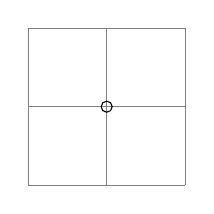
\begin{tikzpicture}
  \draw [help lines] (-1,-1) grid (1,1);
  \coordinate (A) at (0,0);
  \draw (A) circle (2pt);
\end{tikzpicture}
\end{latexcode}

\subsection{坐标系}

有两种坐标系的定义方式:

显式 explicitly: 如 {\ttfamily (canvas cs:x=2, y=0)}

隐式 implicitly: 如笛卡尔坐标 {\ttfamily (2,0)} 或极坐标 {\ttfamily (45:1.5)}

\subsection{循环}

\mint{latex}|\foreach \i [options] in {<list>}{<commands>};|

\begin{latexcode}{nobox}
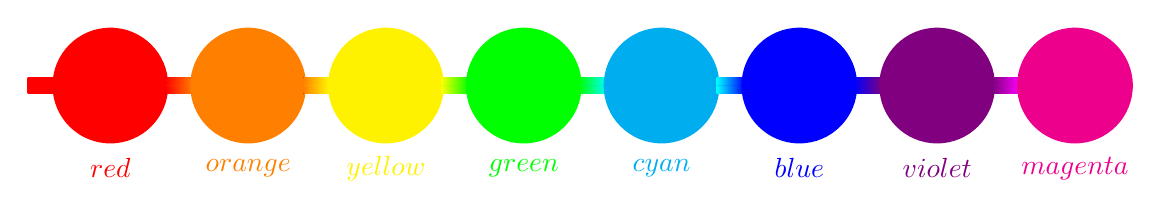
\begin{tikzpicture}[scale=0.35]
  \foreach \rC [count=\j from 0, remember=\rC as \lC (initially red)] in 
  {red, orange, yellow, green, cyan, blue, violet, magenta}{
    \fill[left color=\lC, right color=\rC] (5*\j, -.3) rectangle +(1, .6);
    \fill[\rC] (5*\j, 0) -- ++(3, 0) circle (2.1) node at ++(0, -3) {$\rC$}; 
  }
\end{tikzpicture}
\end{latexcode}

\section{点与曲线}

\subsection{路径 Path 及其属性}

路径 Path 是一些列直线或曲线的点. 创建路径的命令是 {path <specifications>}, 为了使路径可见, 我们需要增加
动作 {\ttfamily draw}\footnote{{draw} 是 {path[draw] 的缩写.}}, 如: 

\begin{latexcode}{nobox}
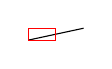
\begin{tikzpicture}
  \path[draw] (0,0) -- (2em,1ex) coordinate (A);
  \path[draw,red] (0,0) rectangle (1em,1ex);
\end{tikzpicture}
\end{latexcode}

{\ttfamily <specifications>} 是一组路径操作或属性, 如:

\begin{tabular}{cc}
\toprule
operations/attributes & descriptions \\
\midrule
{\ttfamily -- (0,0)} & line to \\
{\ttfamily to (0,0)} & line to \\
{\ttfamily let ... in} & 求值运算, 结果存入 {x.}, {y.}, {p.} \\
{\ttfamily [draw]} & 绘图 \\
{\ttfamily color=blue} & 设置颜色 \\
{\ttfamily line width=2pt} & 设置线宽 \\
{\ttfamily coordinate} & 定义点坐标 \\
{\ttfamily node} & 添加文本 (注意不是路径的一部分) \\
{\ttfamily pic} & 引入小的图片和替代 node \\
\bottomrule
\end{tabular}

\begin{latexcode}{nobox}
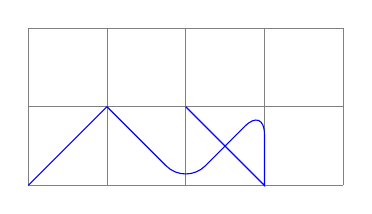
\begin{tikzpicture}
  \draw [help lines] (0,0) grid (4,2);
  \draw[blue] (0,0) -- (1,1) {[rounded corners=10pt] -- (2,0) -- (3,1)}
  -- (3,0) -- (2,1);
\end{tikzpicture}
\end{latexcode}

% \subsection{相对坐标}

% \begin{tabular}{cc}
% \toprule
% form & descriptions \\
% \midrule
% {\ttfamily {-}{-} (x,y)} & 绝对坐标 \\  % {-}{-} 防止变成一个 - 号
% {\ttfamily {-}{-} +(x,y)} & 相对第 1 个绝对坐标 \\
% {\ttfamily {-}{-} ++(x,y)} & 相对前一个坐标 \\
% \bottomrule
% \end{tabular}

% \begin{latexcode}{nobox}
% \begin{tikzpicture}
%   \draw [help lines] (-4,-4) grid (4,4);
%   \draw [-latex] (-4.5,0) -- (4.5,0) node[below] {$x$};
%   \draw [-latex] (0,-4.5) -- (0,4.5) node[left] {$y$};
%   \draw (0,0) node [below left] {$O$};
%   \draw [thick,blue] (0,1) -- (2,1) -- (-2,1.5) -- (-1,-1) -- cycle;
%   \draw [thick,red] (0,1) -- +(2,1) -- +(-2,1.5) -- +(-1,-1) -- cycle; 
%   \draw [thick,green] (0,1) -- ++(2,1) -- ++(-2,1.5) -- ++(-1,-1) -- cycle;
%   \draw [thick,magenta] (0,0) -- ++(-45:1) -- ++(60:2) -- cycle;
% \end{tikzpicture}
% \end{latexcode}

% \subsection{贝塞尔曲线 Bézier}

% \begin{latexcode}{nobox}
% \begin{tikzpicture}
%   \draw [help lines] (0,0) grid (3,3);
%   \draw [thick,blue] (0,0) -- (1,2) .. controls (1.5,3) .. (3,0);
% \end{tikzpicture}
% \end{latexcode}

% \subsection{操作路径 Path}

% {\ttfamily draw, fill, shade, clip} 等

% \section{坐标计算}

% {\ttfamily ($(p1)!c!(p2)$)}

% {\ttfamily ($(p1)!c!angle:(p2)$)}

% 垂直平分线:
% \begin{latexcode}{nobox}
% % \usetikzlibrary{calc}
% \begin{tikzpicture}
%   \coordinate (A) at (0,0);
%   \coordinate (B) at (4,1);
%   \coordinate (M) at ($(A)!0.5!(B)$);
%   \draw (A) -- (B);
%   \draw [blue] ($(M)!2!90:(B)$) -- ($(M)!2!-90:(B)$);
%   \foreach \p in {A,B,M}
%     \draw (\p) circle (2pt);
%   \draw (A) node [below left] {$A$};
%   \draw (B) node [below right] {$B$};
%   \draw (M) node [below right] {$M$};
% \end{tikzpicture}
% \end{latexcode}

% \begin{latexcode}{nobox}
% % \usetikzlibrary{math}
% \begin{tikzpicture}[evaluate={%
%     int \i;
%     for \i in {0, ..., 10}{\r{\i} = .1*(\i+1);}; 
%   }]
%   \foreach \i [evaluate=\i as \tmp using \i*10] in {0,...,10}{% 
%     \filldraw[white, fill=magenta!\tmp!cyan]
%     ($(0, 0)!\i/12!\i*18:(5, -1)$) circle (\r{\i});
%   }
% \end{tikzpicture}
% \end{latexcode}

% \subsection{投影}

% {\ttfamily ($(p1)!p!(p2)$)}

% 三角形的高线:
% \begin{latexcode}{nobox}
% % \usetikzlibrary{calc}
% \begin{tikzpicture}
%   \coordinate (A) at (0,0);
%   \coordinate (B) at (5,-1);
%   \coordinate (C) at (2,3);
%   \draw[thick] (A) -- (B) -- (C) -- cycle;
%   \draw[blue,thin] 
%     (A) -- ($(B)!(A)!(C)$) coordinate (A')
%     (B) -- ($(A)!(B)!(C)$) coordinate (B')
%     (C) -- ($(A)!(C)!(B)$) coordinate (C');
%   \foreach \p in {A,B,C,A',B',C'}
%     \draw (\p) circle (2pt);
%   \draw (A) node [below left] {$A$};
%   \draw (B) node [below right] {$B$};
%   \draw (C) node [above] {$C$};
%   \draw (A') node [above right] {$A'$};
%   \draw (B') node [above left] {$B'$};
%   \draw (C') node [below] {$C'$};
% \end{tikzpicture}
% \end{latexcode}

% Simson 线:
% \begin{latexcode}{nobox}
% % \usetikzlibrary{calc}
% \begin{tikzpicture}
%   \coordinate (A) at (-10:2);
%   \coordinate (B) at (55:2);
%   \coordinate (C) at (170:2);
%   \coordinate (P) at (-80:2);
%   \draw [magenta] (0,0) circle (2);
%   \draw[thick] (A) -- (B) -- (C) -- cycle;
%   \draw[blue,thin] 
%     (P) -- ($(B)!(P)!(C)$) coordinate (A')
%     (P) -- ($(A)!(P)!(C)$) coordinate (B')
%     (P) -- ($(A)!(P)!(B)$) coordinate (C');
%   \draw[red,thick] (A') -- (C');
%   \foreach \p in {A,B,C,A',B',C',P}
%     \draw (\p) circle (2pt);
%   \draw (A) node [right] {$A$};
%   \draw (B) node [above right] {$B$};
%   \draw (C) node [left] {$C$};
%   \draw (A') node [above] {$A'$};
%   \draw (B') node [above right] {$B'$};
%   \draw (C') node [above right] {$C'$};
%   \draw (P) node [below right] {$P$};
% \end{tikzpicture}
% \end{latexcode}

% \subsection{交点}

% \subsubsection*{第 1 形式}

% \mint{latex}|name intersections={of=<curve1> and <curve2>, name=<prefix>}|

% 如果有非封闭图形, 可以作为排序的图形 {\ttfamily sort by=curve name}:

% \begin{latexcode}{nobox}
% \begin{tikzpicture}
%   \draw [help lines] (-2,-2) grid (2,2);
%   \draw [name path=circle] (0,0) circle (2);
%   \draw [name path=line] (-2,-2) -- (3,0);
%   \path [name intersections={of=circle and line, name=iP, sort by=line}];
%     \foreach \j/\pos in {1/below, 2/below right}{%
%   \filldraw[red] (iP-\j) circle (2pt) node[\pos, black] {$I_{\j}$}; }
% \end{tikzpicture}
% \end{latexcode}

% \subsubsection*{第 2 形式}\mint{latex}|name intersections={of=<curve1> and <curve2>, by=<points>}|

% \begin{latexcode}{nobox}
% \begin{tikzpicture}
%   \draw [help lines] (-2,-2) grid (2,2);
%   \draw [name path=circle] (0,0) circle (2);
%   \draw [name path=curve] (-2,-2) .. controls (-0.5,-1) .. (0,0)
%     .. controls (0.5,1) .. (2,2);
%   \path[name intersections={of=circle and curve, by={A, B}, sort by=curve}];
%   \foreach \P/\pos in {A/below, B/above}{%
%     \filldraw[blue] (\P) circle (2pt) node[\pos] {$\P$};
%   }
% \end{tikzpicture}
% \end{latexcode}

% \subsubsection*{第 3 形式}\mint{latex}|name intersections={of=<curve1> and <curve2>, name=<prefix>, total=\t}|

% \begin{tikzpicture}
%   \draw[help lines] (-2,-2) grid (2,2);
%   \draw[name path=circle] (0,0) circle (2);
%   \draw[rotate=-45,name path=ellipse] (-1,-1) ellipse (3 and 1);
%   \fill[name intersections={of=circle and ellipse, name=I, total=\t}] 
%     [blue] \foreach \j in {1, ..., \t}{%
%       (I-\j) circle (2pt) node[above right] {$I_\j$} 
%     };
% \end{tikzpicture}

% \section{几何变换}

% 几何变换有:

% \begin{itemize}
%   \item {\ttfamily rotate=<angle in degree>}
%   \item {\ttfamily xshift=<length, yshift=<length>}
%   \item {\ttfamily shift=<\{vector\}>} 注意花括号
%   \item {\ttfamily xscale=<factor>, yscale=<factor>}
%   \item {\ttfamily scale=<factor>}
% \end{itemize}

% \begin{latexcode}{nobox}
% \begin{tikzpicture}
%   \draw[help lines] (-2,-2) grid (4,4);
%   \draw[thick,blue] 
%     (-1,0) -- (0,0) -- (60:1) .. controls (1,0) .. (2,0);
%   \draw[thick,red,rotate=45] 
%     (-1,0) -- (0,0) -- (60:1) .. controls (1,0) .. (2,0);
%   \draw[thick,orange,shift={(2,.5)}] 
%     (-1,0) -- (0,0) -- (60:1) .. controls (1,0) .. (2,0);
%   \draw[thick,cyan,rotate=45,shift={(2,.5)}] 
%     (-1,0) -- (0,0) -- (60:1) .. controls (1,0) .. (2,0);
%   \draw[thick,magenta,shift={(2,.5)},rotate=45] 
%     (-1,0) -- (0,0) -- (60:1) .. controls (1,0) .. (2,0);
% \end{tikzpicture}
% \end{latexcode}

% \section{箭头}

% \tikz \draw[->] (0,0) -- (1,0);

% \tikz \draw[-latex] (0,0) -- (1,0);

% \section{Node}

% A node is typically a rectangle or circle or another simple shape with some text on it. Nodes are added to paths using the special path operation {\ttfamily node}. {\itshape Nodes are not part of the path itself}. Rather, they are added to the picture just before (with the attribute {\ttfamily behind path}) or after the path has been drawn.

% Coordinate transformations do not apply to a node. Its anchor remains the same. To achieve a translation for example, the shift command must be placed inside the node’s name parentheses.

% \subsection{定义 Node}

% Thepathoperation...node[<options>] (nName) at (a,b) {content}...;createsanode for the current path, i.e. writes down the content at the point (a,b) with some node options and name nName. The node options or attributes have no effect outside the node; they control its

% \begin{itemize}
%   \item position with respect to the elements of the path – anchor
%   \item appearance
%   \item label.
% \end{itemize}

% \begin{latexcode}{nobox}
% \begin{tikzpicture}
%   \path (0, 0) coordinate (A) node[below left] {$A$}; 
%   \path (3, 2) coordinate (B) node[below right] {$B$}; 
%   \draw (A) to[out=-30, in=180] 
%     node[draw, red, pos=.5, above left] {content}
%     node[draw, blue, pos=.5] {content} (B); 
%   \draw[fill=white] (A) circle (2pt) (B) circle (2pt);
% \end{tikzpicture}
% \end{latexcode}

% \section{plot}

% {\ttfamily addplot, addplot3} 需要 pgfplots 宏.

% \subsection{从文件中读取数据}

% \begin{latexcode}{nobox}
% \begin{tikzpicture}
%   \begin{axis}
%   \addplot table [x=column 1, y=column 2, col sep=comma] {table.csv};
%   \end{axis}
% \end{tikzpicture}
% \end{latexcode}

% \subsection{绘制函数图像}

% 可以使用 {\ttfamily plot} , 可以使用 {\ttfamily addplot} \footnote{\url{https://pressbooks.bccampus.ca/introtolatex/chapter/packages/}}:

% \begin{latexcode}{nobox}
% \begin{tikzpicture}
%   \draw[help lines] (-4,-4) grid (4,4);
%   \draw[-latex] (-4.5,0) -- (4.5,0) node [below] {$x$};
%   \draw[-latex] (0,-4.5) -- (0,4.5) node [left] {$y$};
%   \draw (0,0) node [below left] {$O$};
%   \draw[domain=-3:3, smooth, variable=\x, red] 
%     plot ({\x}, {\x*\x/5}) node[above] {$y=\cfrac{x^2}{5}$};
%   \draw[domain=-3:3, samples=20, variable=\x, blue] 
%     plot ({\x}, {-cos(2*deg(\x))-1}) node[above] {$y=-\cos{2x}-1$};
%   \draw[variable=\t, domain=-1.6:1.6, samples=50]
%     plot (\t*\t-1, {\t*(\t*\t-1)}) node[above] {$y^2=x^3+x^2$};
% \end{tikzpicture}
% \end{latexcode}

% \begin{latexcode}{nobox}
% \begin{tikzpicture}
%   \begin{axis}[
%     axis lines = left,
%     xlabel = $x$,
%     ylabel = {$f(x)$}
%   ]
%   \addplot [ 
%     domain=-10:10,
%     samples=30,
%     color=blue
%   ]{x^2 + 2*x + 1};
%   \addplot [ 
%     domain=-10:10,
%     samples=40,
%     color=red
%   ]{20*sin(pi*x^2)};
%   \end{axis}
% \end{tikzpicture}
% \end{latexcode}

% \subsection{三维图}

% \begin{latexcode}{nobox}
% \begin{tikzpicture}[scale=2]
%   \begin{axis}[
%     %title={$f(x,y)=y\exp(-x^2-\|y\|)$},
%     hide axis,
%     colormap/cool,  
%   ]
%   \addplot3[
%     surf, 
%     domain=-3:3, 
%     domain y=-3:3, 
%     samples=40
%   ]{y*exp(-x*x-abs(y))};
%   \end{axis}
% \end{tikzpicture}
% \end{latexcode}

% \begin{latexcode}{nobox}
% \begin{tikzpicture}[scale=2]
%   \begin{axis}[
%     %title={$f(x,y)=\cfrac{\sin{\sqrt{x^2+y^2}}}{\sqrt{x^2+y^2}}$},
%     hide axis,
%     colormap/cool,
%   ]
%   \addplot3[
%     mesh,
%     samples=50,
%     domain=-8:8,
%   ]{sin(deg(sqrt(x^2+y^2)))/sqrt(x^2+y^2)};
%   \end{axis}
% \end{tikzpicture}
% \end{latexcode}

% \section{pic}

% \subsection{标记角}

% \begin{latexcode}{nobox}
% \begin{tikzpicture}
%   \draw
%     (3,-1) coordinate (a) node[right] {$A$}
%     -- (0,0) coordinate (b) node[left] {$B$}
%     -- (2,2) coordinate (c) node[above right] {$C$}
%     pic["$\alpha$", draw=orange, <->, angle eccentricity=1.2, angle radius=1cm]
%     {angle=a--b--c};
% \end{tikzpicture}
% \end{latexcode}




\backmatter

\cleardoublepage
\addtocontents{toc}{\bigskip}

\bibliography{references}

\printindex % 索引

\end{document}